%%%%%%%%%%%%%%%%%%%%%%%%%%%%%%%%%%%%%%%%%%%%%%%%%%%%%%%%%%%%%
%LUNGHEZZA STIMATA 3-4 FACCIATE DI TESTO PER GIORNATA DI LAB%
%%%%%%%%%%%%%%%%%%%%%%%%%%%%%%%%%%%%%%%%%%%%%%%%%%%%%%%%%%%%%
%%%%IN TOTALE CIRCA 15 FACCIATE DI TESTO IMMAGINI ESCLUSE%%%%
%%%%%%%%%%%%%%%%%%%%%%%%%%%%%%%%%%%%%%%%%%%%%%%%%%%%%%%%%%%%%
%Di solito nei papers accademici / tecnici si usa sempre
%la forma impersonale, quindi "E' stata misurata la corrente..."
%oppure "si è proceduto a misurare la corrente...."
%anziché "Abbiamo misurato la corrente..."

\documentclass[journal]{IEEEtran}

% *** CITATION PACKAGES ***
\usepackage[style=ieee]{biblatex} 
\bibliography{analog.bib}    %your file created using JabRef
\usepackage{hyperref}
% *** MATH PACKAGES ***
\usepackage{amsmath}
 \usepackage{multirow}

% *** PDF, URL AND HYPERLINK PACKAGES ***
\usepackage{url}
\usepackage{makeidx}
% correct bad hyphenation here
\hyphenation{op-tical net-works semi-conduc-tor}
\usepackage{graphicx}  %needed to include png, eps figures
\usepackage{float}  % used to fix location of images i.e.\begin{figure}[H]
\makeindex

\begin{document}

% paper title
\title{Laboratorio di elettronica analogica\\ 
%\small{1 gennaio 2020}
}

% author names 
\author{\begin{center}Matteo Barbagiovanni\textsuperscript{1},
        Stefano Barbero\textsuperscript{2},
        Federico Malnati\textsuperscript{3},
        Valerio Pagliarino\textsuperscript{4},
        {\small \\
        \textsuperscript{1}
        matteo.barbagiovanni@edu.unito.it -
        \textsuperscript{2}
        stefano.barbero376@edu.unito.it
        \textsuperscript{3}
        federico.malnati@edu.unito.it -
        \textsuperscript{4}
        valerio.pagliarino@edu.unito.it}
        \end{center}}% <-this % stops a space
        
% The report headers
\markboth{Università degli Studi di Torino - C.d.L. Triennale in Fisica - 21/10/21 - A.A. 2021-2022    \quad   \quad \quad \quad   \quad \quad \quad  \quad   \quad \quad \quad   \quad \quad LABORATORIO DI ELETTRONICA \quad \quad }%do not delete next lines
{Shell \MakeLowercase{\textit{et al.}}: Bare Demo of IEEEtran.cls for IEEE Journals}

% make the title area
\maketitle

% As a general rule, do not put math, special symbols or citations
% in the abstract or keywords.
\begin{abstract}  
Oggi la ricerca in fisica in qualunque ambito è supportata in modo fondamentale dall'elettronica e dall'informatica che permettono l'acquisizione dei dati, la loro analisi e l'esecuzione di simulazioni; l'elettronica digitale ha rivoluzionato le tecniche di calcolo, ma l'elettronica analogica continua ad essere cruciale, poiché interviene nel processo di trasduzione dell'osservabile fisica in un segnale elettrico e nel condizionamento di quest'ultimo fino alla conversione in digitale ad opera di \textit{ADCs}, \textit{TDCs} o altri sistemi. Non stupisce allora il fatto che in molti sistemi di misura e rivelazione l'elettronica analogica rappresenti il vero limite alle prestazioni dell'apparato. In questa relazione di laboratorio verranno analizzati alcuni circuiti analogici di rilievo per la strumentazione fisica: dopo una breve introduzione agli strumenti e lo studio qualitativo di un raddrizzatore a singola semionda realizzato con diodo al silicio, si prenderanno in esame alcune applicazioni degli amplificatori operazionali. Dapprima si verificherà il funzionamento in configurazione ad anello aperto come discriminatore di soglia e verrà misurato lo \textit{slew rate}, dopodiché si passerà ad alcune configurazioni retroazionate che consentono l'amplificazione dei segnali con guadagno prefissato e il calcolo di operazioni matematiche tra segnali analogici come integrali, derivate, somme e differenze. Successivamente verrà realizzato mediante due amplificatori operazionali un comparatore con isteresi (trigger di Schmitt) in grado di discriminare un segnale a cui è stato sommato del rumore mediante il secondo stadio analogico. Si concluderà questa relazione con l'analisi di un semplice circuito di read-out per un fotomoltiplicatore al silicio (SiPM) che consentirà di calcolare il guadagno del sensore e con alcune verifiche delle leggi di propagazione dei segnali su linee coassiali.
%Concluso, da rileggere
\end{abstract}

%%%%%%%%%%%%%%%%%%%%%%%%%%%%%%%%%%%%%%%%%%
\section{Strumentazione utilizzata} %Valerio

\IEEEPARstart{I}{} circuiti qui descritti sono stati implementati mediante l'uso di componentistica \textit{COTS} \textit{(off the shelf} in standard \textit{through hole}, più maneggevole rispetto a quella \textit{SMD}, installata su breadboard. Le interconnessioni sono state realizzate con normali jumper mentre le alimentazioni sono state collegate utilizzando connettori a banana. I segnali sono stati misurati con l'oscilloscopio utilizzando sonde passive attenuate X10.
Segue oltre una brevissima dei principali strumenti di misura e genearatori utilizzati.

\subsection{\textbf{Oscilloscopio Tektronix TBS1104}}

\begin{figure}[h!]
  \centering
  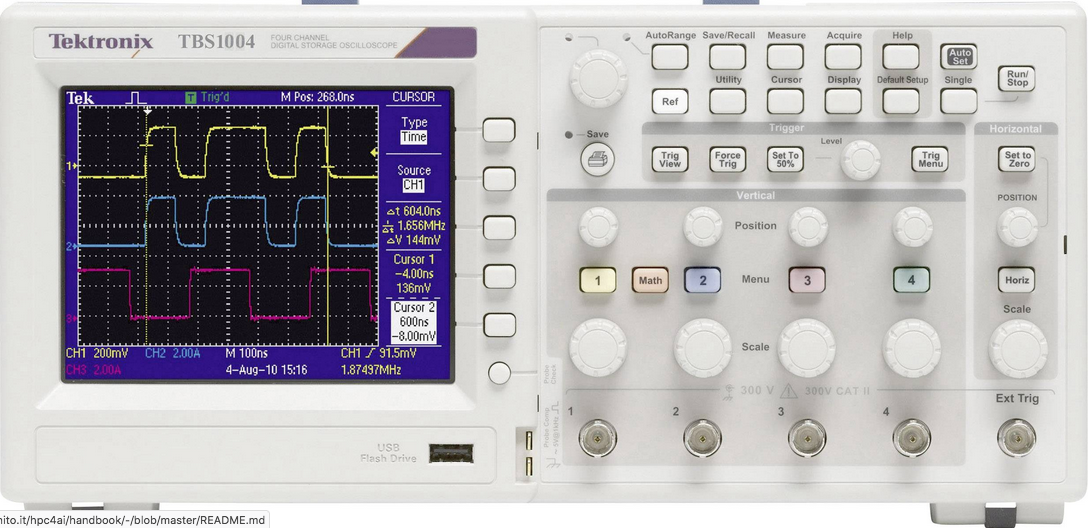
\includegraphics[width=0.18\textwidth]{lab-reports/Schematics-and-graphics/TEK Osc.png}
\end{figure}

La maggior parte delle misure di tensione e tempo è stata realizzata con un \textit{digital storage oscilloscope (DSO)} Tektronix 1104 con banda passante di 70 MHz, frequenza di campionamento massima di 1 GSa/s che consente fino a 5 ns/div di risoluzione temporale, 4 canali e 2.5K punti di memoria per finestra di acquisizione, risoluzione verticale di 8 bit e sensibilità fino a 10 mV/div.

\subsection{\textbf{Oscilloscopio Rhode & Schwartz}}

\begin{figure}[h!]
  \centering
  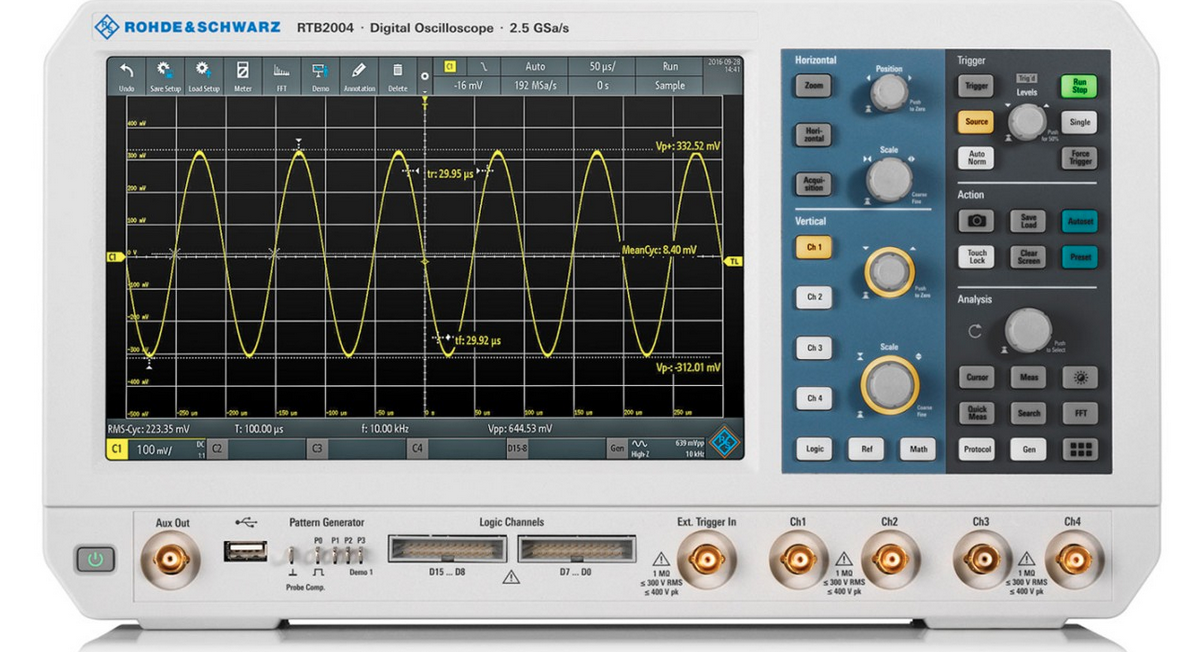
\includegraphics[width=0.18\textwidth]{lab-reports/Schematics-and-graphics/RS Osc.png}
\end{figure}

Per visualizzare il segnale in uscita dal fotomoltiplicatore al silicio è stata invece utilizzato un oscilloscopio di fascia più alta Rhode & Schwarz RTB2004 dotato di un ADC a 10 bit con banda passante di 70 MHz e frequenza di campionamento massima di 2.5 GSa/s che consente raggiungere una risoluzione temporale di 1 ns/div. Quest'ultima caratteristica, unita alla sensibilità fino a 1 mV/div, ha permesso di visualizzare correttamente i segnali molto deboli e veloci prodotti dal sensore quando viene eccitata una singola cella.

\subsection{\textbf{Generatori di funzioni Rigol DG1022Z e Siglent SDG1010}}

\begin{figure}[h!]
  \centering
  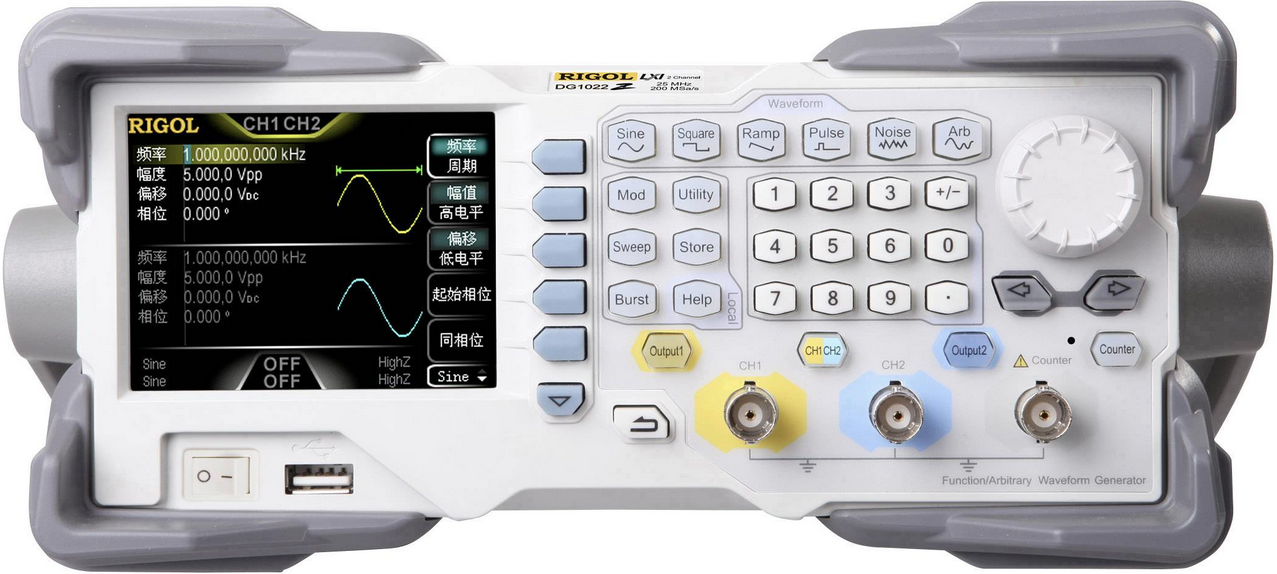
\includegraphics[width=0.18\textwidth]{lab-reports/Schematics-and-graphics/RIGOL Gen.png}
\end{figure}

\begin{figure}[h!]
  \centering
  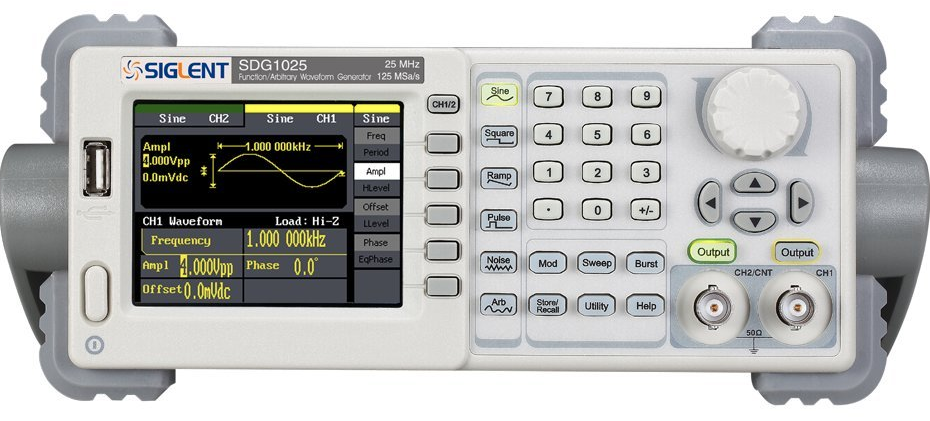
\includegraphics[width=0.18\textwidth]{lab-reports/Schematics-and-graphics/SIGLENT Gen.png}
\end{figure}

Questi due generatori di segnali arbitrari basati sulla sintesi digitale diretta (DDS) sono stati impiegati per il pilotaggio dei circuiti. Il secondo dispositivo è stato impiegato per la generazione dell'impulso di tensione per l'alimentazione del led nell'esperienza di caratterizzazione del SiPM, mentre il primo apparecchio per tutte le altre misure. Il generatore \textit{Rigol} ha una banda passante massima di 25 MHz, una frequenza di campionamento del DAC di 100 MSa/s e una risoluzione verticale di 14 bit. Il generatore \textit{Siglent}, invece, ha una banda passante di 10 MHz, una frequenza di campionamento del DAC di 125 MSa/s, una risoluzione verticale anch'esso di 14 bit e supporta la generazione di impulsi mediante la velocità "burst" con un fronte di salita / discesa minimo di 7 ns e una durata minima di 16 ns. Il generatore dispone di un'uscita di sincronismo in standard TTL con durata degli impulsi > 50 ns che abbiamo utilizzato per pilotare il trigger esterno dell'oscilloscopio Rhode & Schwarz.

\subsection{\textbf{Generatore di impulsi veloci Keithley 3390}}

\begin{figure}[h!]
  \centering
  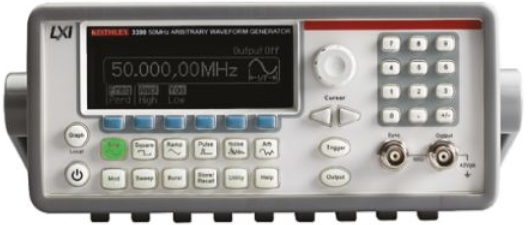
\includegraphics[width=0.18\textwidth]{lab-reports/Schematics-and-graphics/KEIT Gen.png}
\end{figure}


Per lo studio della propagazione di segnali attraverso una linea di trasmissione coassiale è stato fondamentale disporre di un generatore di segnali in grado di produrre impulsi sufficientemente veloci, in relazione al tempo di propagazione lungo la linea, con fronti più ripidi possibile. Per questo motivo è stato impiegato un generatore di segnali arbitrari Keithley 3390, anch'esso basato sulla tecnologia della sintesi digitale diretta, che dispone di una banda passante analogica di 50 MHz, una durata minima degli impulsi di 20 ns e un fronte di salita minimo di 10 ns.

\subsection{\textbf{Multimetro digitale Meterman 35XP e alimentatore da banco duale GW-Instek GPS-4303}}
Il corredo di strumentazione è stato completato con multimetro digitale Meterman 35XP utilizzato per misurare tensioni, resistenze e capacità, soprattutto in fase montaggio e verifica dei circuiti e da un generatore di tensione GW-Instek GPS-4303 con 4 canali a tensione e corrente variabile utilizzabili per fornire alimentazione duale all'amplificatore operazionale impiegato. Il multimetro ha una risoluzione di 3-3/4 cifre, un'accuratezza nelle misure di tensione DC di 0.5 \% della lettura + 1 * ultima cifra fino a 1KV e un'accuratezza nelle misure di resistenza di 1.0 \% della lettura + 4 * ultima cifra fino a 40 M$\Omega$. Per l'accuratezza nelle misure di capacità si rimanda al datasheet. L'alimentatore è invece in grado di fornire sui canali utilizzati fino a 30V / 5A.

%%%%%%%%%%%%%%%%%%%%%%%%%%%%%%%%%%%%%%%%%%
\section{\textbf{Ponte raddrizzatore a diodi a singola semionda}} %Matteo
\subsection{\textbf{Introduzione all'esperienza}}
In molteplici applicazioni si ha la necessità di convertire tensioni alternate in tensioni continue (AC/DC). Uno dei modi più immediati per ottenere tale risultato è quello di sfruttare raddrizzatori non controllati, quali raddrizzatori a singola/doppia semi-onda, a ponte monofase/trifase o esafase.
I diodi a giunzione p-n sono dei componenti elettronici passivi non lineari, il cui funzionamento è regolato dalla struttura cristallina delle due giunzioni, le quali saranno rispettivamente di tipo \textit{n} (drogati con atomi pentavalenti, che comporta un eccesso di elettroni) e di tipo \textit{p} (eccesso di lacune). Nei pressi del punto di contatto tra le due si formerà una \textit{regione di svuotamento}, grazie alla combinazione tra elettroni e lacune, che creerà una barriera di potenziale. I diodi presentano dunque due possibilità di impiego. Una delle quali è la \textit{polarizzazione diretta}, in cui il polo positivo del generatore è collegato al terminale di
tipo \textit{p}. In questa configurazione la regione di svuotamento si ridurrà fino a permettere il passaggio di corrente. La forma funzionale della corrente in funzione della tensione sarà descritta dalla \textit{funzione di Shockley}: \[I_{D} = I_{0}(e^{V/\eta V_T}-1)\] dove $I_{0}$ rappresenta la corrente di saturazione inversa, il termine $V_{T}$ è il potenziale di Einstein, dipendente dalla temperatura e $\eta$ è il fattore di idealità dipendente dal materiale costituente del diodo.
\begin{figure}[H]%[!ht]
\begin {center}
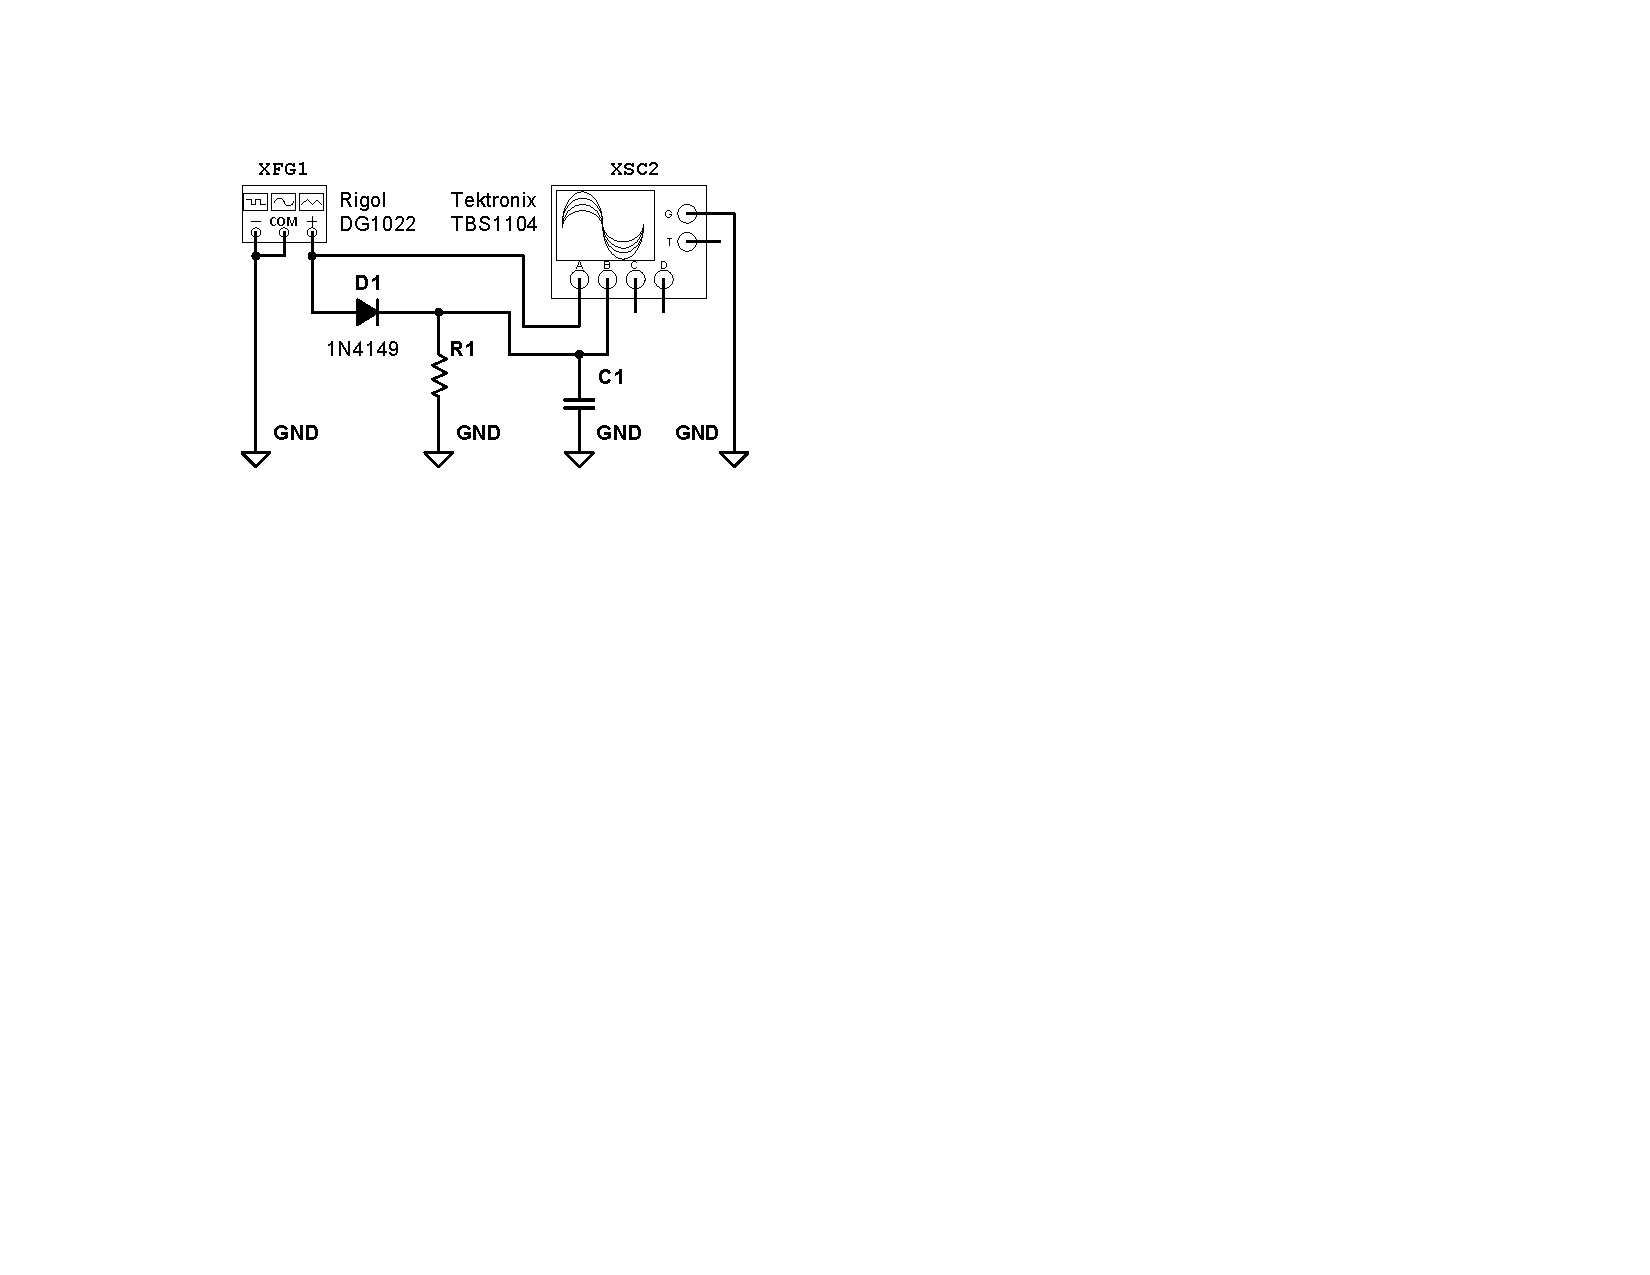
\includegraphics[width=0.38\textwidth]{sch-simulations/output/Diode-rectifier.pdf}
\caption{Didascalia}
\label{fig:oscilloscope}
\end {center}
\end{figure}
La trattazione successiva riguarda i raddrizzatori a singola semi-onda ed in particolare l'implementazione del circuito in \texit{Fig. 1}, realizzato tramite un unico diodo più un condensatore di filtraggio. In tale configurazione durante la fase di crescita del segnale in ingresso $V_{in}$ il condensatore agisce da accumulatore permettendo alla $V_{out}$ di copiare la tensione in entrata. Nel secondo quarto di periodo, il diodo passa in interdizione a causa del condensatore che si scarica lentamente rispetto alla variazione dell'ingresso. Infine durante la fase di OFF del diodo l'usicta è determinata unicamente dalla scarica del condensatore sulla resistenza.
Quindi in regime di funzionamento il diodo rimane acceso per un periodo $\Delta T$ in cui avviene la fase di carica e la tensione di uscita passa dal suo valore minimo al suo valore massimo. Un raddrizzatore ben funzionante fa si che la \textit{tensione di ripple} sia la minore possibile e ciò è strettamente correlato al valore della costante di tempo $\tau$.
Analizzando il funzionamento del circuito in assenza del condensatore di livellamento invece si avrà in uscita un segnale costituito solamente dalla semi-onda positiva, nel caso di \textit{polarizzazione diretta}, oppure della semi-onda negativa in \textit{polarizzazione inversa} come viene evidenziato dalla \texit{Fig. 2}.
\begin{figure}[H]%[!ht]
\begin {center}
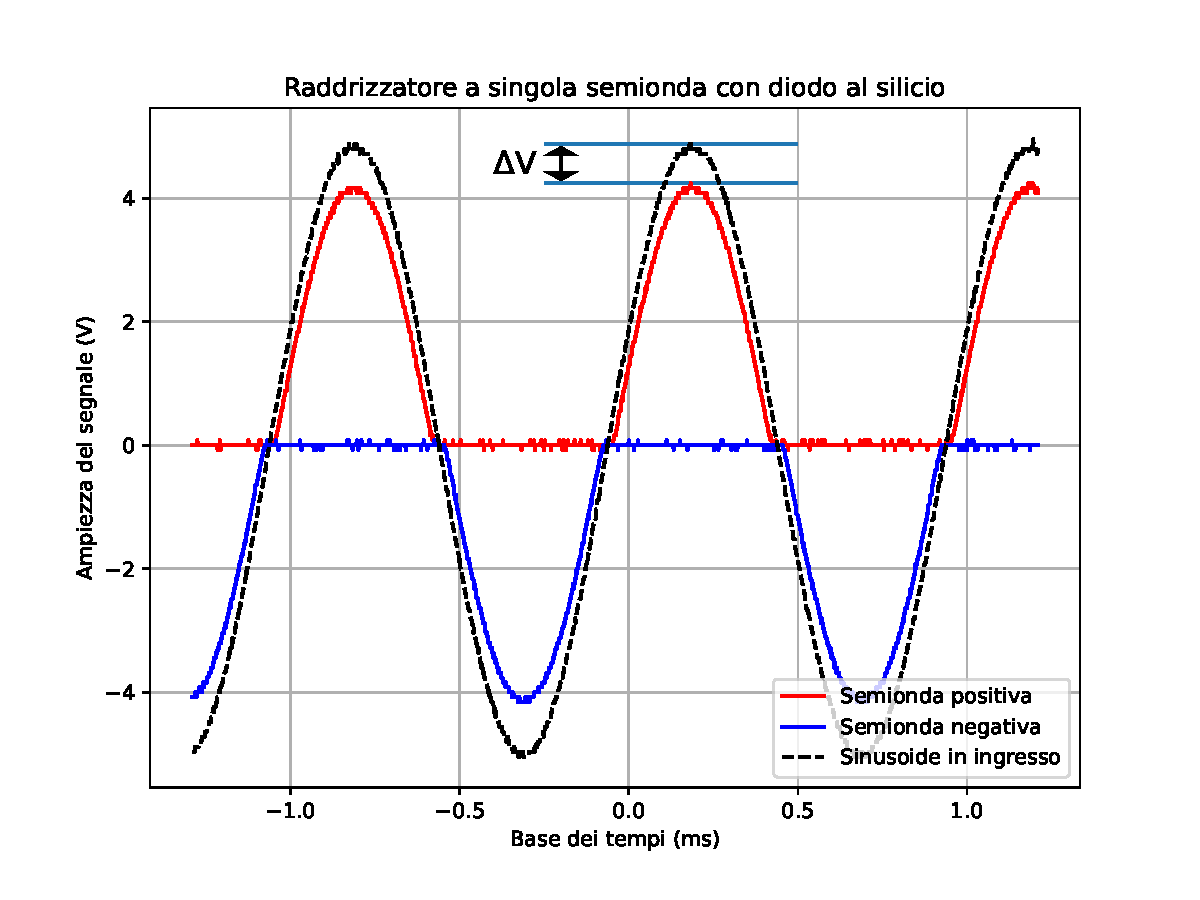
\includegraphics[width=0.38\textwidth]{analysis/output/half-wave-rectifier.pdf}
\caption{Didascalia}
\label{fig:oscilloscope}
\end {center}
\end{figure}
\[\Delta V = 0.64 V \] 
Ricordando che in letteratura il valore della \textit{tensione di soglia} per i diodi al Silicio è pari a $V_{\gamma}=0.6V$ e considerando possibili impurità del diodo in questione si evince un totale accordo col dato empirico. Tale supposizione è sostenuta dal risultato del \textit{Test di Gauss} ($Z = 0.071$).




\subsection{\textbf{Introduzione all'esperienza}}
Descrizione

\subsection{\textbf{Componentistica e circuito}}
Descrizione

\subsection{\textbf{Caratterizzazione}}
Descrizione

\subsection{\textbf{Discussione dei risultati}}
Descrizione


%%%%%%%%%%%%%%%%%%%%%%%%%%%%%%%%%%%%%%%%%%
\section{\textbf{Introduzione all'amplificatore operazionale}}
Passiamo ora allo studio una serie di circuiti notevoli di amplificazione, confronto ed esecuzione di operazioni matematiche sui segnali realizzati con amplificatori operazionali. Questi componenti sono altamente versatili e sono utilizzati in quasi tutti gli ambiti in cui è necessario il condizionamento di un segnale analogico. Sono modellizzabili come amplificatori differenziali (OPA) con impedenza in ingresso teoricamente infinita, impedenza di uscita teoricamente nulla, banda passante infinita e guadagno a circuito aperto teoricamente infinito. Nella realizzazione pratica è possibile raggiungere per queste grandezze valori molto grandi o molto piccoli grazie all'utilizzo di processi di fabbricazione integrati che consentono di realizzare su un singolo die circuiti analogici complessi multistadio (almeno stadio di ingresso differenziale, stadio di guadagno, stadio di uscita). Nelle esperienze che seguiranno verranno utilizzati OPA \textbf{LM741} prodotti dalla Texas Instruments con package DIP, dispositivi a basso costo alimentati in tensione duale $\pm$ 15 V con \textit{slew rate} tipico di 0.5 V/$\mu$s, larghezza di banda di 1.5 MHz e guadagno tipico per grandi segnali a T = 298 K di 50 V/mV.

%%%%%%%%%%%%%%%%%%%%%%%%%%%%%%%%%%%%%%%%%%
\section{\textbf{Anello aperto invertente (zero-crossing detector)}} %Stefano
Descrizione

\begin{figure}[H]%[!ht]
\begin {center}
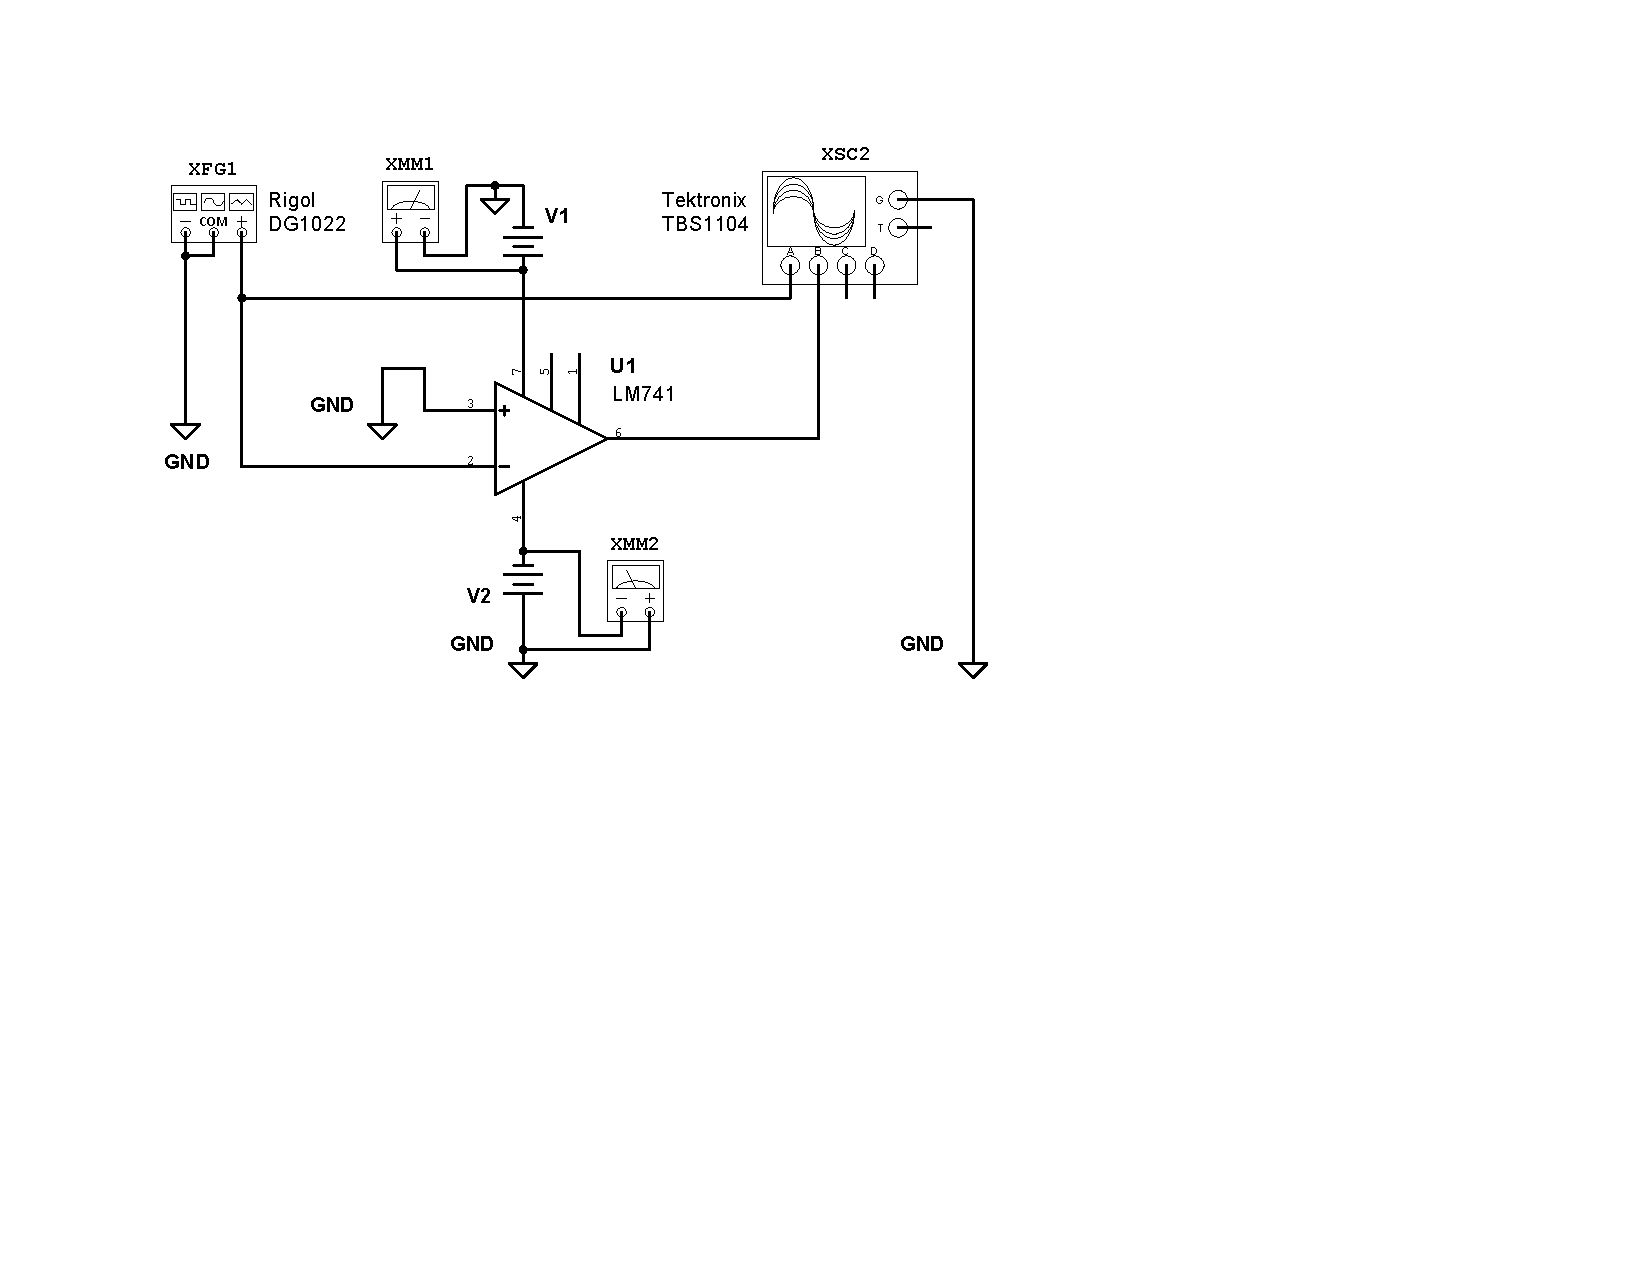
\includegraphics[width=0.38\textwidth]{sch-simulations/output/OPA-open-loop-inverting.pdf}
\caption{Didascalia}
\label{fig:oscilloscope}
\end {center}
\end{figure}


%%%%%%%%%%%%%%%%%%%%%%%%%%%%%%%%%%%%%%%%%%
\section{\textbf{Anello aperto non invertente}} %Stefano
Descrizione

\begin{figure}[H]%[!ht]
\begin {center}
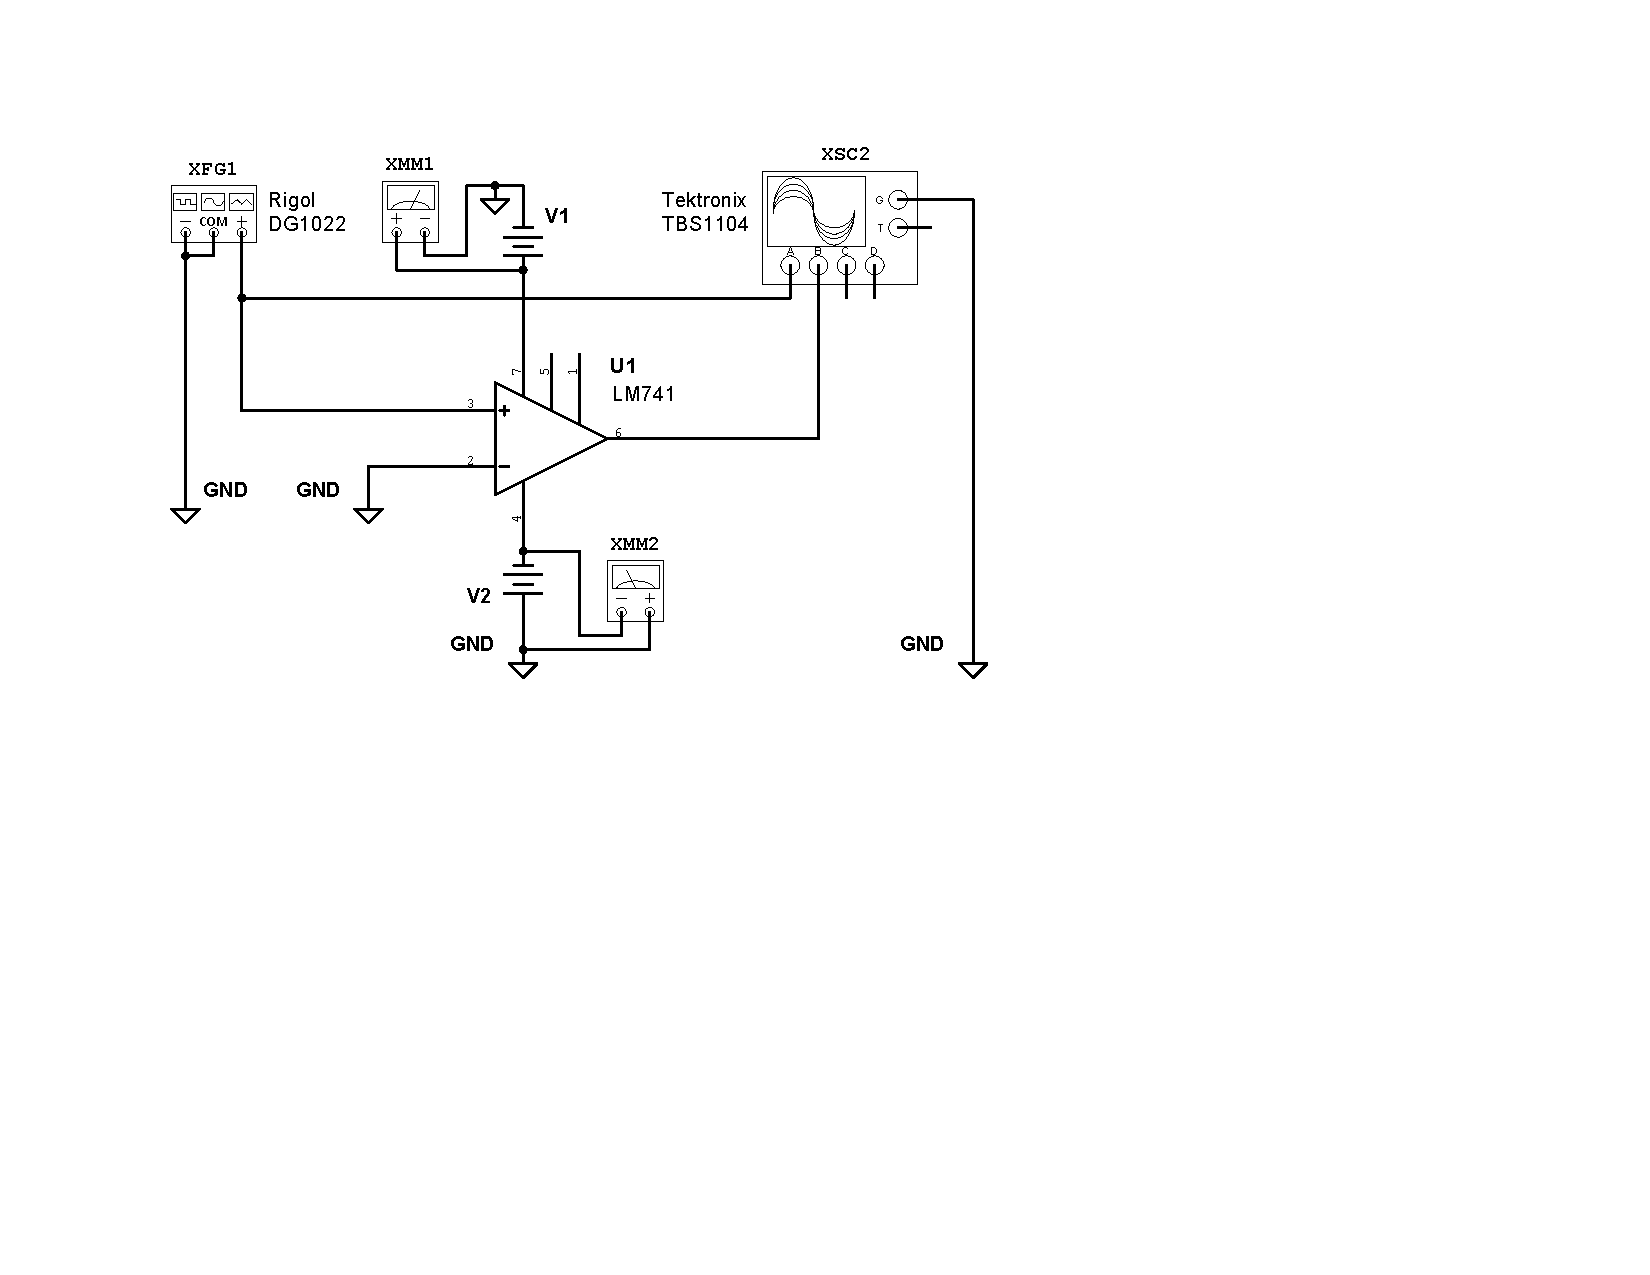
\includegraphics[width=0.38\textwidth]{sch-simulations/output/OPA-open-loop-non-inverting.pdf}
\caption{Didascalia}
\label{fig:oscilloscope}
\end {center}
\end{figure}


%%%%%%%%%%%%%%%%%%%%%%%%%%%%%%%%%%%%%%%%%%
\section{\textbf{Amplificatore reazionato invertente}} %Stefano
Descrizione

\begin{figure}[H]%[!ht]
\begin {center}
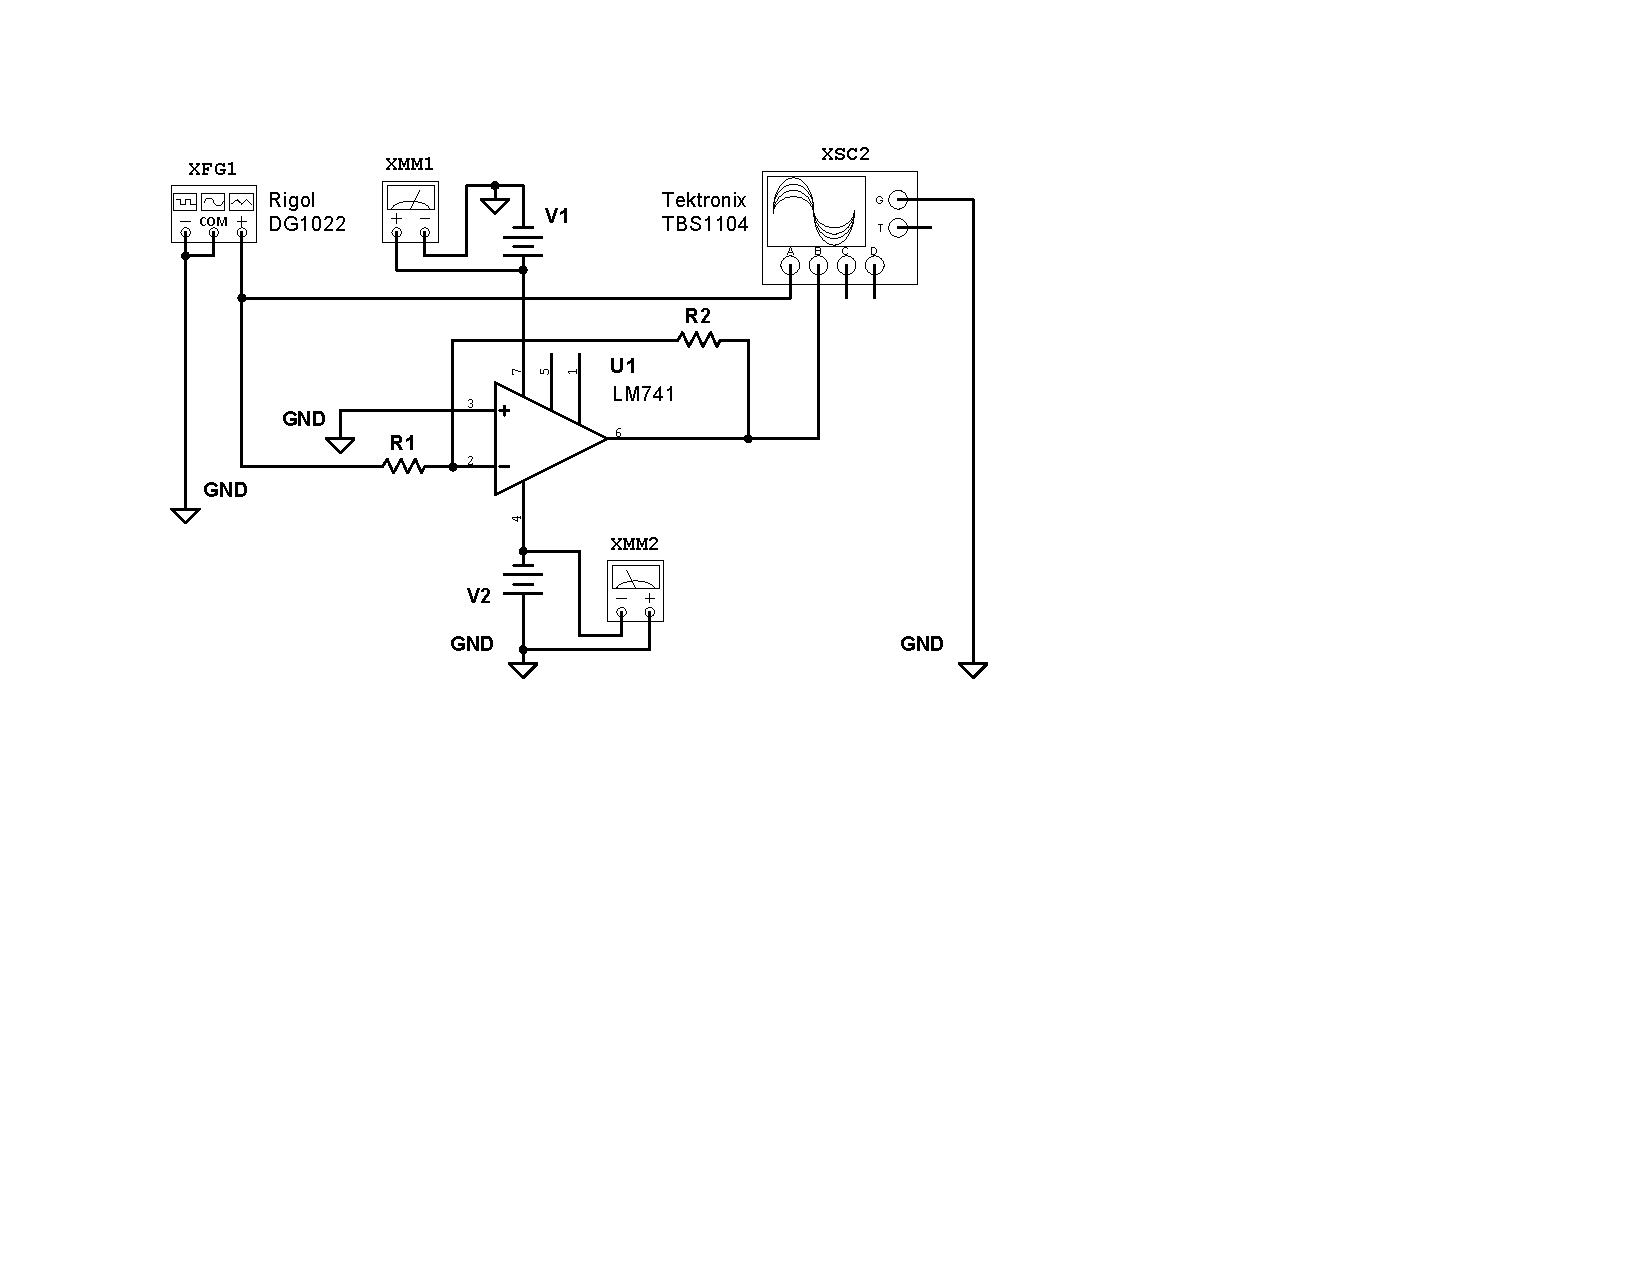
\includegraphics[width=0.38\textwidth]{sch-simulations/output/OPA-closed-loop-inverting.pdf}
\caption{Didascalia}
\label{fig:oscilloscope}
\end {center}
\end{figure}

\subsection{Studio della risposta in frequenza}


%%%%%%%%%%%%%%%%%%%%%%%%%%%%%%%%%%%%%%%%%%
\section{\textbf{Amplificatore reazionato non invertente}} %Matteo
\subsection{\textbf{Introduzione all'esperienza}}
\begin{figure}[H]%[!ht]
\begin {center}
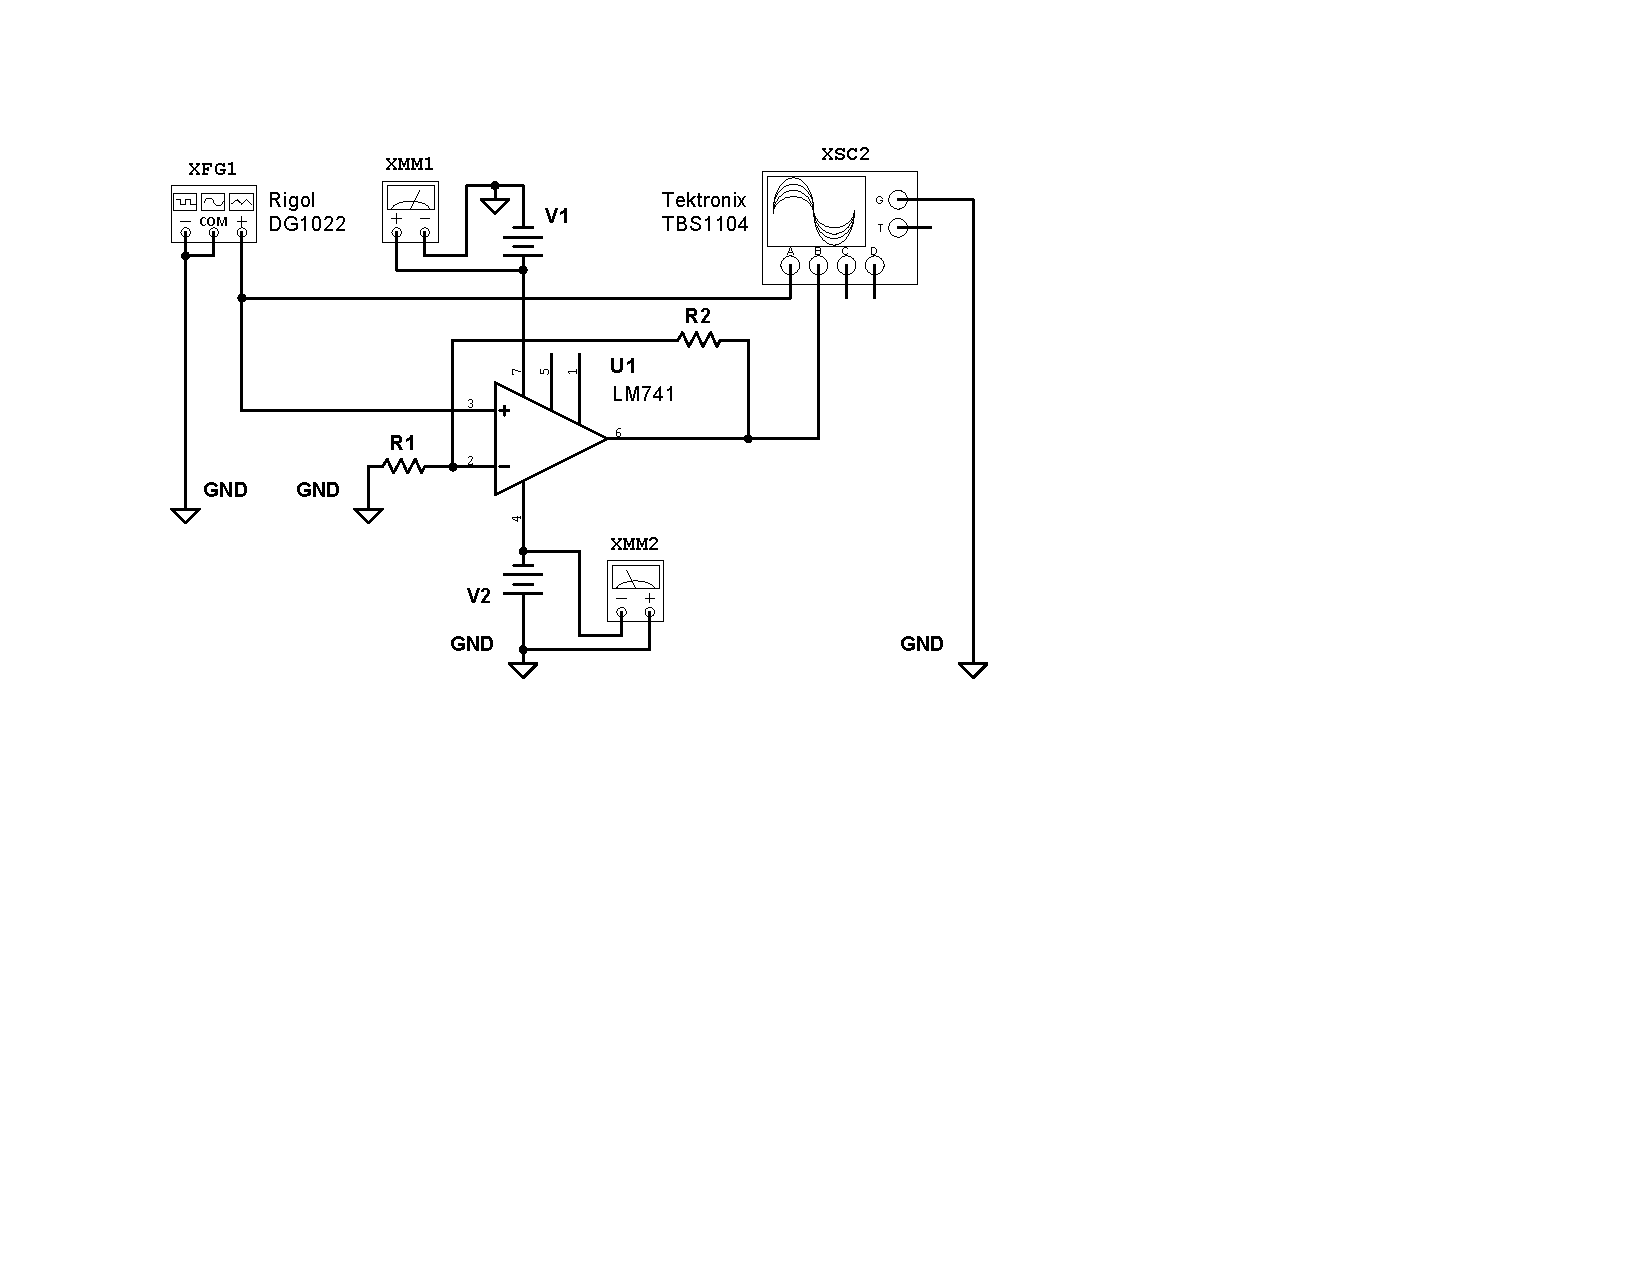
\includegraphics[width=0.38\textwidth]{sch-simulations/output/OPA-closed-loop-non-inverting.pdf}
\caption{Didascalia}
\label{fig:oscilloscope}
\end {center}
\end{figure}
Un amplificatore non invertente ha la peculiarità di dare in uscita un segnale proporzionale a quello d'ingresso e in fase con esso. Il segnale è applicato all'ingresso non invertente affinché il guadagno $A$ sia positivo. Infatti per l'equipotenzialità degli ingressi si ha: \[V_{-} = V_{+} = V_{i}\] \[V_{-} = \frac{R_1}{R_1+R_2}=V_{+}\] \[V_{o}=(1+\frac{R_2}{R_1}V_{+}\]
da cui si ricava che $A=\frac{V_{o}}{V_i}=1+\frac{R_2}{R_1}$.
\subsection{\textbf{Caratterizzazione}}
Sono state selezionati diversi resistori in maniera tale da esaminare più casi di amplificazione. Nel primo caso $R_1=\Omega$ e $R_2=\Omega$ in maniera da tale da attendersi un guadagno di circa due volte. Si è proceduto con la presa dati della risposta in frequenza del circuito. I dati sono stati successivamente fittati attraverso l'utilizzo di una funzione di transfer caratterizzata da tre poli:
\[H(s)=\frac{k}{(1+as)(1+bs)(1+cs)}\] 
per poi estrarre il valore della $H.F.$

\begin{figure}[H]%[!ht]
\begin {center}
\includegraphics[width=0.38\textwidth]{analysis/output/OPA-bode}
\caption{Didascalia}
\label{fig:oscilloscope}
\end {center}
\end{figure}


\subsection{Studio della risposta in frequenza}

\subsection{Slew rate}

%%%%%%%%%%%%%%%%%%%%%%%%%%%%%%%%%%%%%%%%%%
\section{Discriminatore ad anello aperto con soglia arbitraria} %Stefano

\begin{figure}[H]%[!ht]
\begin {center}
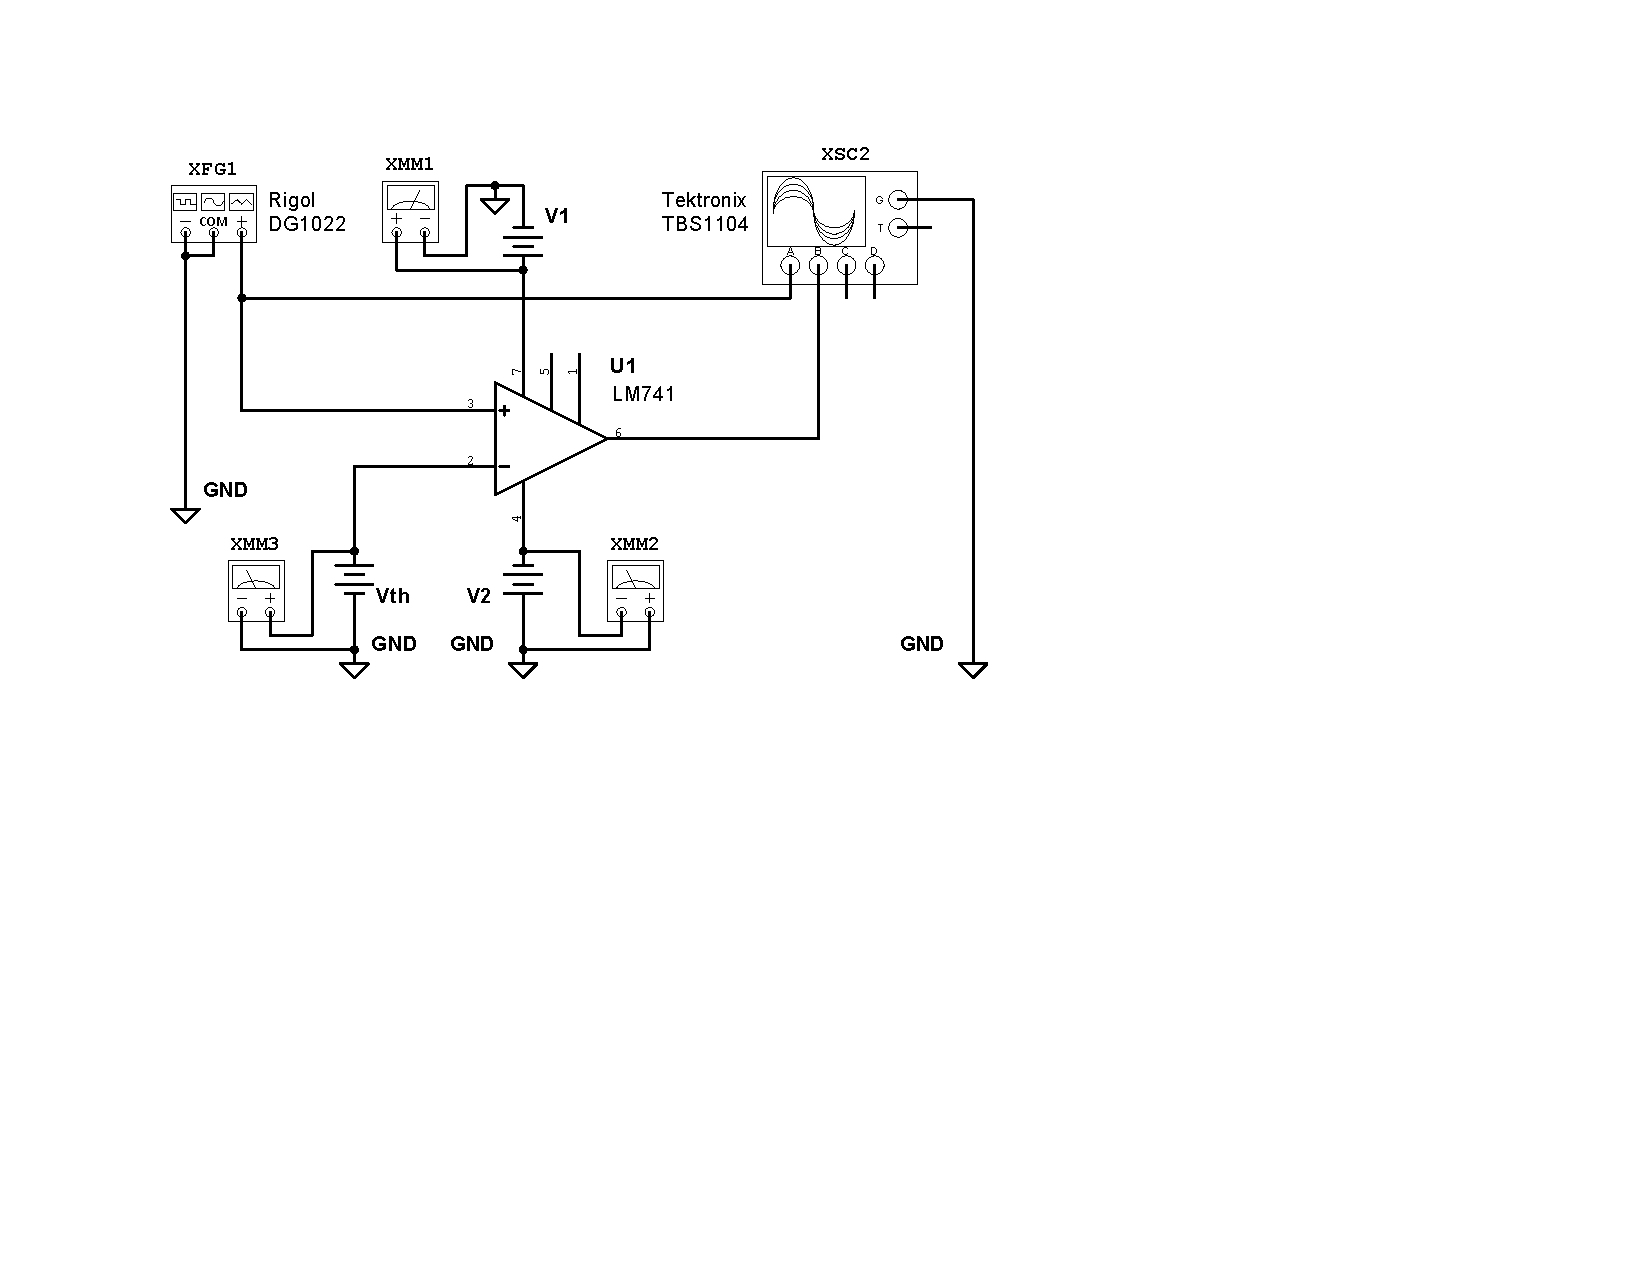
\includegraphics[width=0.38\textwidth]{sch-simulations/output/OPA-biased.pdf}
\caption{Didascalia}
\label{fig:oscilloscope}
\end {center}
\end{figure}

%%%%%%%%%%FINE PRIMO GIORNO%%%%%%%%%%%%%%%
%%%%%%%%%%INIZIO SECONDO GIORNO%%%%%%%%%%%

%%%%%%%%%%%%%%%%%%%%%%%%%%%%%%%%%%%%%%%%%%
\section{Amplificatore logaritmico} %Stefano

\begin{figure}[H]%[!ht]
\begin {center}
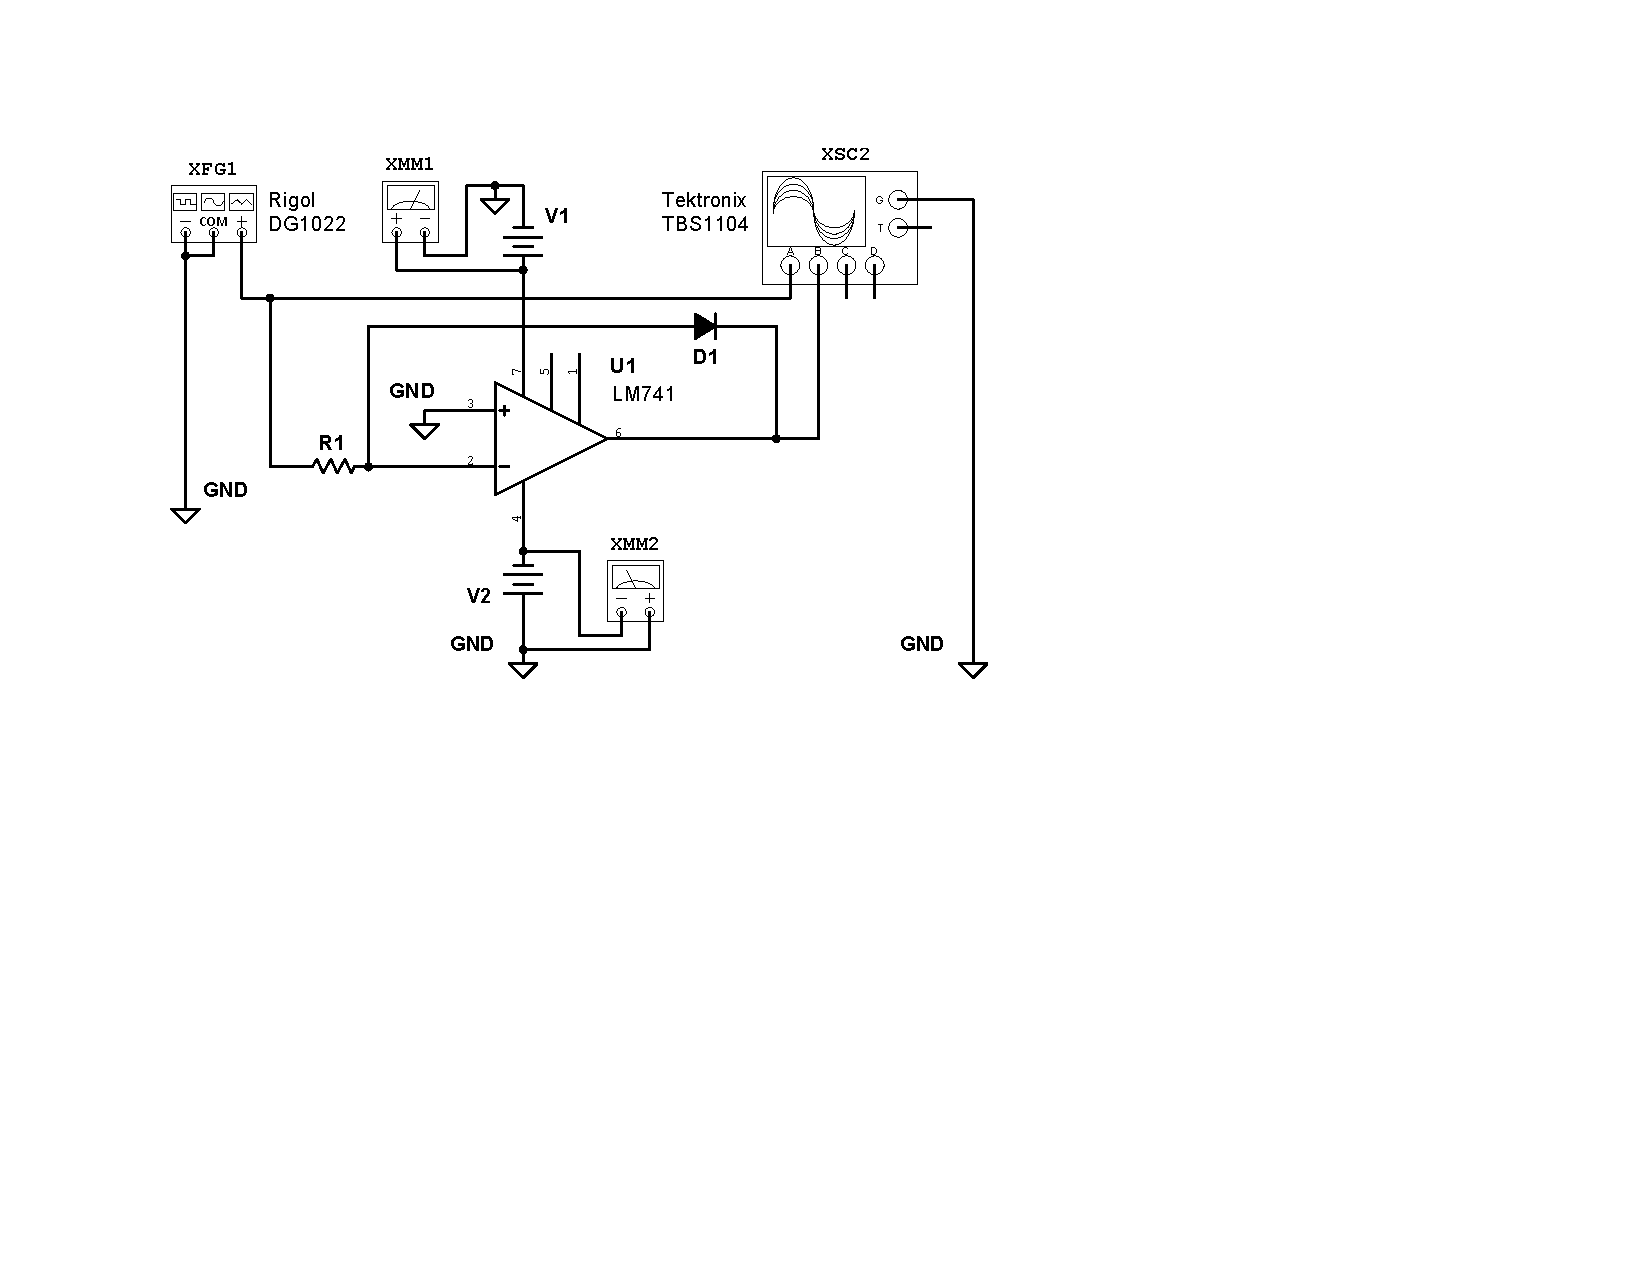
\includegraphics[width=0.38\textwidth]{sch-simulations/output/OPA-log.pdf}
\caption{Didascalia}
\label{fig:oscilloscope}
\end {center}
\end{figure}

%%%%%%%%%%%%%%%%%%%%%%%%%%%%%%%%%%%%%%%%%%
\section{Grafico di risposta}


%%%%%%%%%%%%%%%%%%%%%%%%%%%%%%%%%%%%%%%%%%
\section{Amplificatore integratore reale invertente} %Matteo
\subsection{\textbf{Introduzione all'esperienza}}
In questa esperienza di laboratorio verrà analizzato il funzionamento di un \textit{OPA integratore}, osservandone in primo luogo la risposta a diversi tipi di segnali, quali a gradino, rampa e sinusoidali, per poi studiarne il comportamento in funzione della variazione di frequenza della $V_{in}$.
\subsection{\textbf{circuito}}
\begin{figure}[H]%[!ht]
\begin {center}
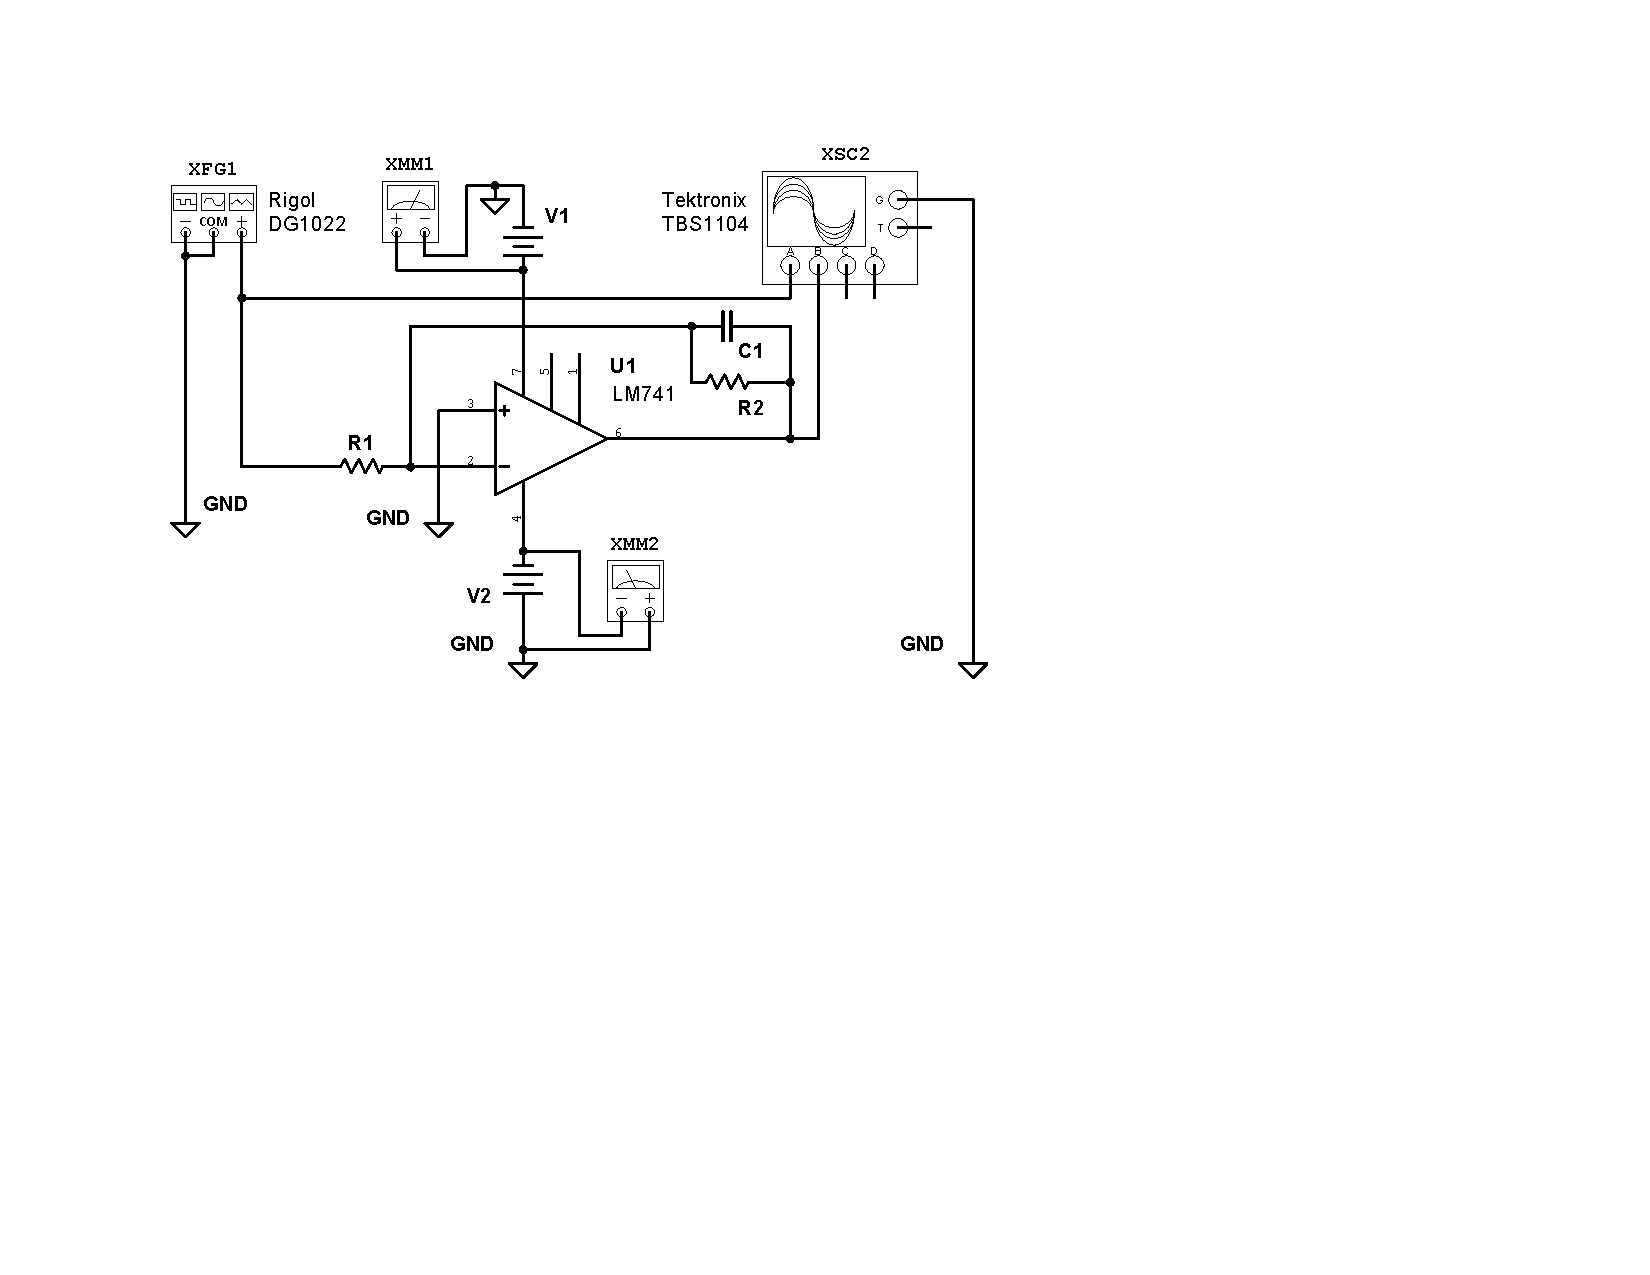
\includegraphics[width=0.38\textwidth]{sch-simulations/output/OPA-integratore.pdf}
\caption{Didascalia}
\label{fig:oscilloscope}
\end {center}
\end{figure}
Come sottintende il nome, l'Op-Amp integratore è un operazionale che esegue l'operazione matematica dell'integrazione, facendo si che il circuito emetta una $V_{out}$ proporzionale all'integrale della $V_{in}$. In altre parole, facendo riferimento alla \textit{Fig.9}, l'ampiezza del segnale in uscita è determinato dal periodo di tempo in cui una tensione è presente in input, poiché la corrente attraverso il circuito di feedback carica o scarica il condensatore mentre il feedback negativo richiesto avviene attraverso il condensatore.
Affinchè l'amplificatore non vada in saturazione alle basse frequenze è stato aggiunto in parallelo a $C$ un resistore $R_{2}$. Ciò fa si che a fequenze limitate, essendo il periodo della tensione in ingresso relativamente lungo, il condensatore si commporti come una impedenza infinita, determinando un guadagno $A_{v}=-R_{2}/R{1}$. In questa configurazione si parla infatti di \textit{integratore limitato}. 
Un fattore importante è che il circuito si comporta effettivamente da integratore solo per frequenze superiori a quella di taglio, $f_{t}=\frac{1}{2 \pi C R_{1} }$, per cui buona norma per ottenere un circuito efficiente è quella di scegliere $R$ e $C$ in maniera consona ai propri obiettivi. 
\subsection{\textbf{Caratterizzazione}}
Inizialmente si sono scelte $R$ e $C$ con lo scopo di ottenere una frequenza di taglio non eccessivamente bassa per favorire lo studio della risposta in frequenza della fase successiva: \[f_{t} = \frac{1}{2 \pi R_{1} C}= 685.63 \pm 44.13 Hz\] 

\begin{figure}[H]%[!ht]
\begin {center}
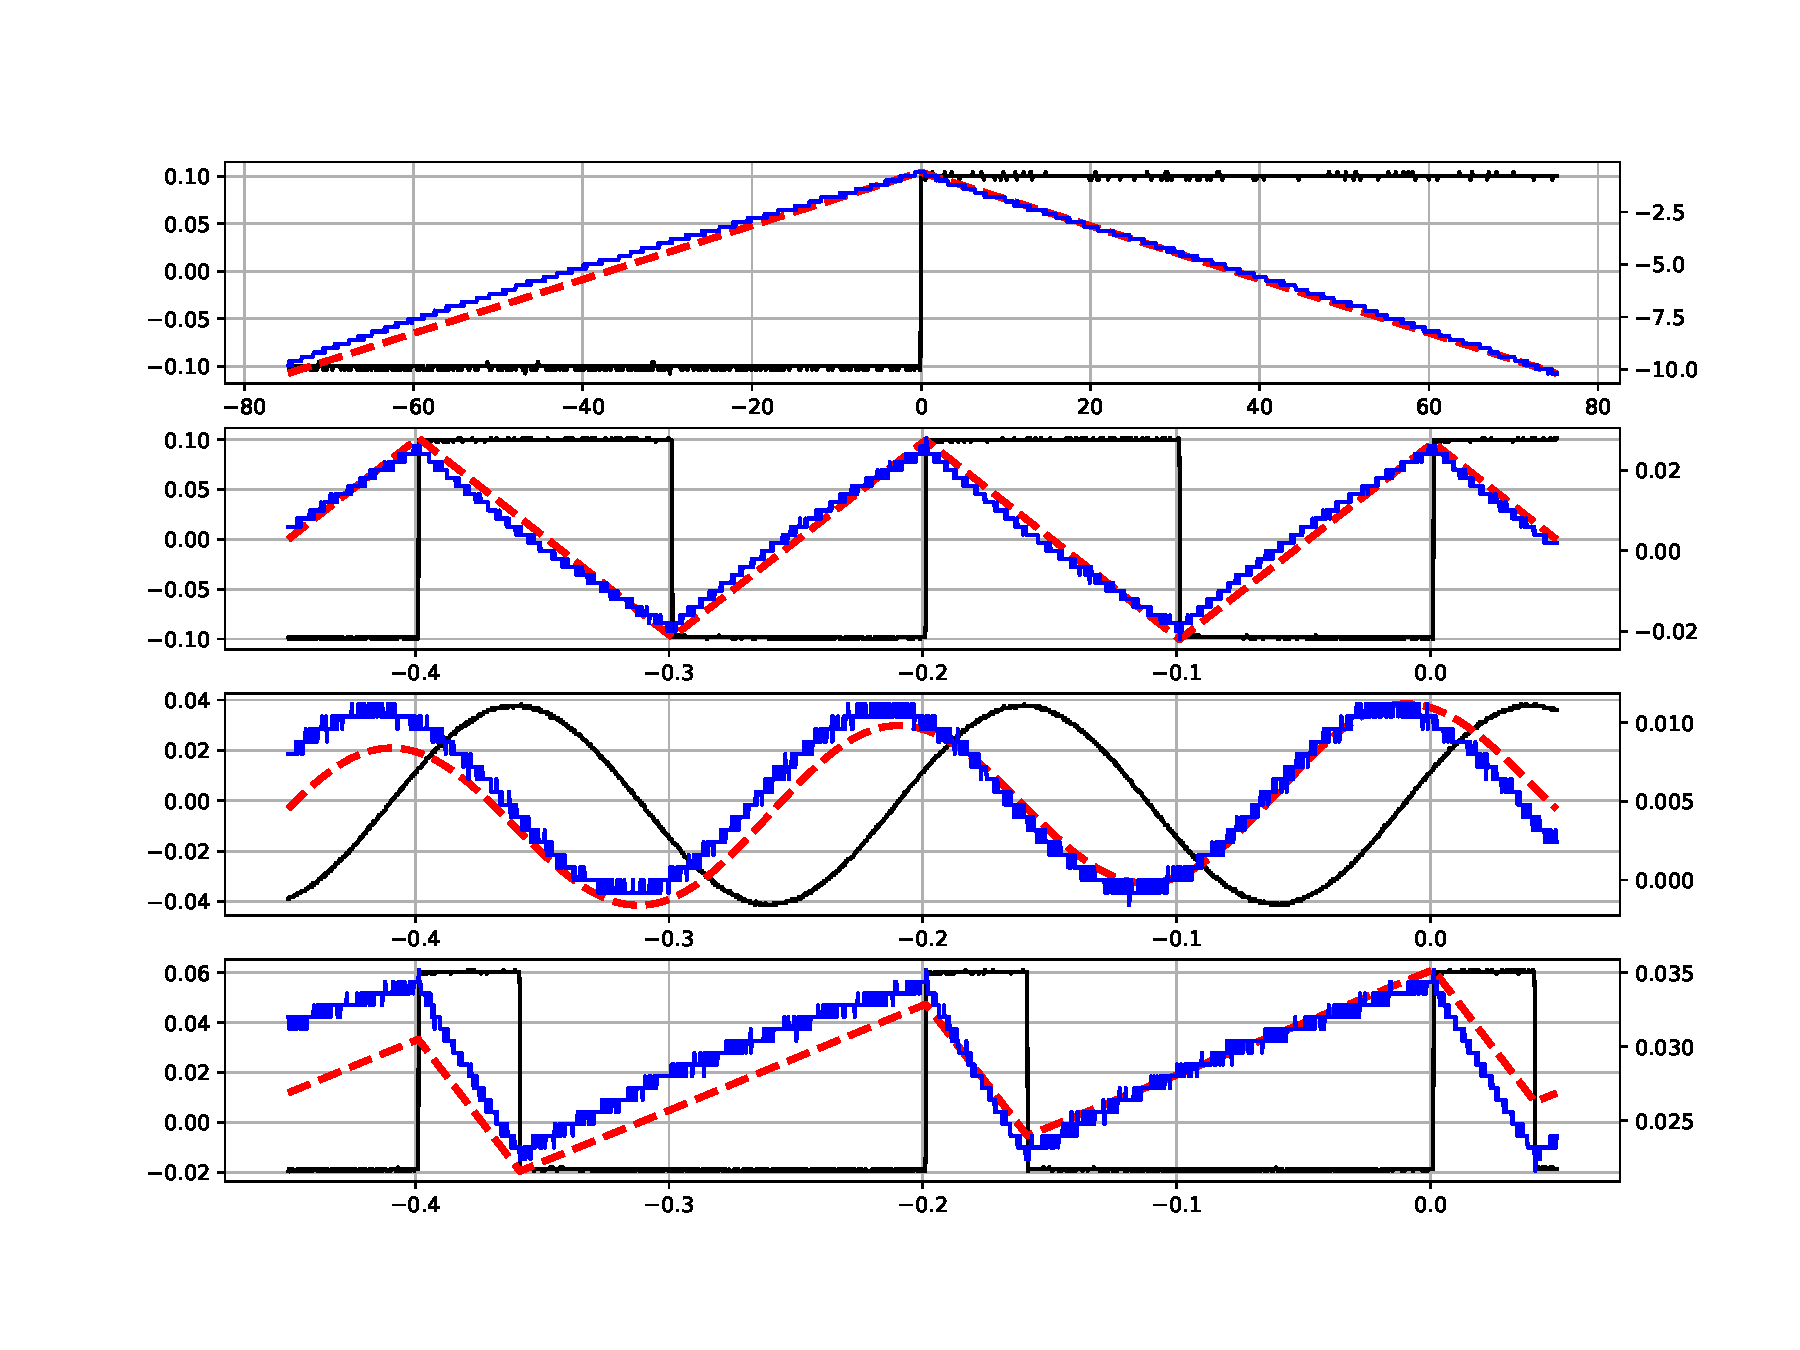
\includegraphics[width=0.38\textwidth]{analysis/output/OPA-integ-with-res.pdf}
\caption{Didascalia}
\label{fig:oscilloscope}
\end {center}
\end{figure}
Impostando una frequenza, $f=valore_da _controllare$, si è proceduto con l'osservazione della risposta del circuito, \textit{Fig. 10}. Come atteso la $V_{out}$ risulta essere molto vicina all'integrale del segnale in ingresso. In particolare si nota l'affinità con l'integrale calcolato numericamente rappresentato dalla linea rossa tratteggiata.
Terminata la prima fase si è passati all'analisi della output del circuito in funzione della frequenza. I dati sono stati graficati e fittati in primo luogo con la forma funzionale di un filtro passa basso e poi in seguito attraverso la trasformata di Laplace della funzione di transfer: \[H(s)=k/(as+1)^2\] con polo doppio in corrispondenza di $f=685 Hz$ valore pienamente compatibile con la frequenza di taglio.
\begin{figure}[H]%[!ht]
\begin {center}
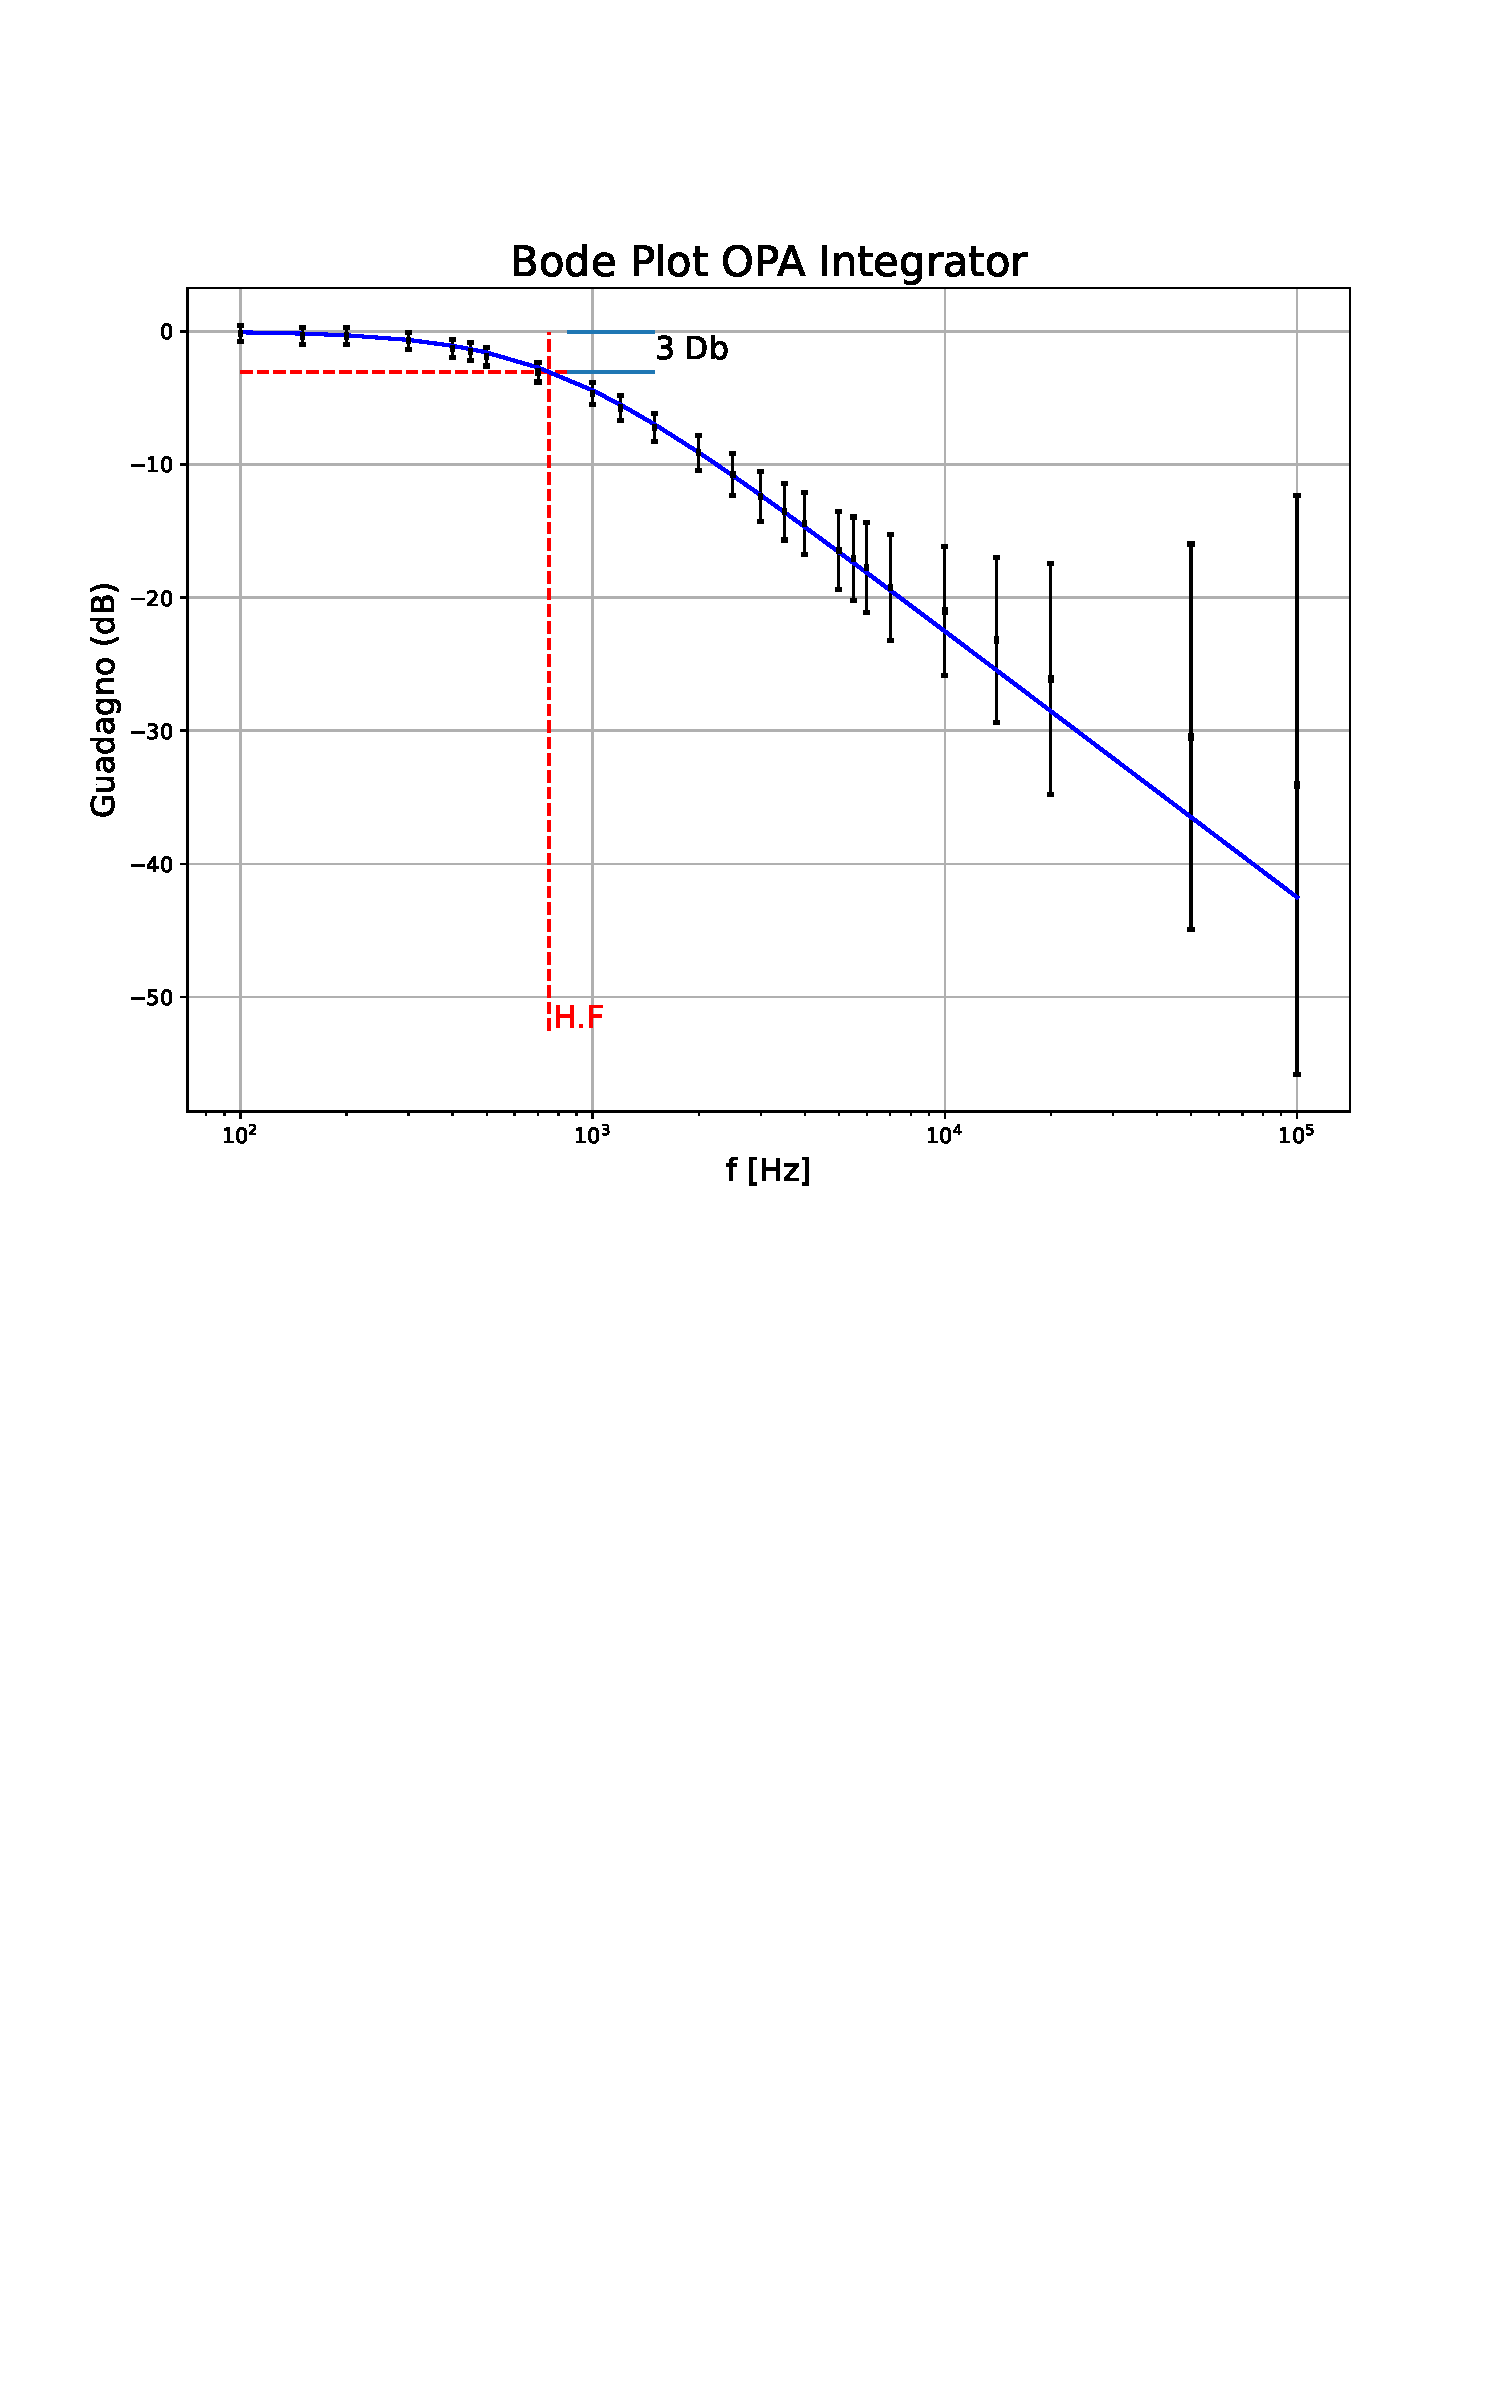
\includegraphics[width=0.38\textwidth]{analysis/output/OPA-integrator_bode(mag).pdf}
\caption{Didascalia}
\label{fig:oscilloscope}
\end {center}
\end{figure}
Dalla forma funzionale ottenuta è poi stato estratto il valore della $H.F. = 418.28892698398096 Hz$ (serve trovare modo per estrarre errore per poi confrontarlo con frequenza di taglio).
Infine facendo la regressione del fit è stato ricavato il valore di \textit{magnitude} relativo alla frequenza nulla, $A_{v}(0)=-0.317$ ed è stato confrontato col valore ricavato dall'espressione, derivata dalla letteratura, $A_{v} = 20log_{10}(-R_{2}/R{1}) = -0.142 \pm 0.397 $. La misura empirica risulta consistente con quella teorica ($Z=0.44$).
%%%%%%%%%%%%%%%%%%%%%%%%%%%%%%%%%%%%%%%%%%
\section{Diagramma di Bode}


%%%%%%%%%%%%%%%%%%%%%%%%%%%%%%%%%%%%%%%%%%
\section{Amplificatore derivatore} %Matteo

\begin{figure}[H]%[!ht]
\begin {center}
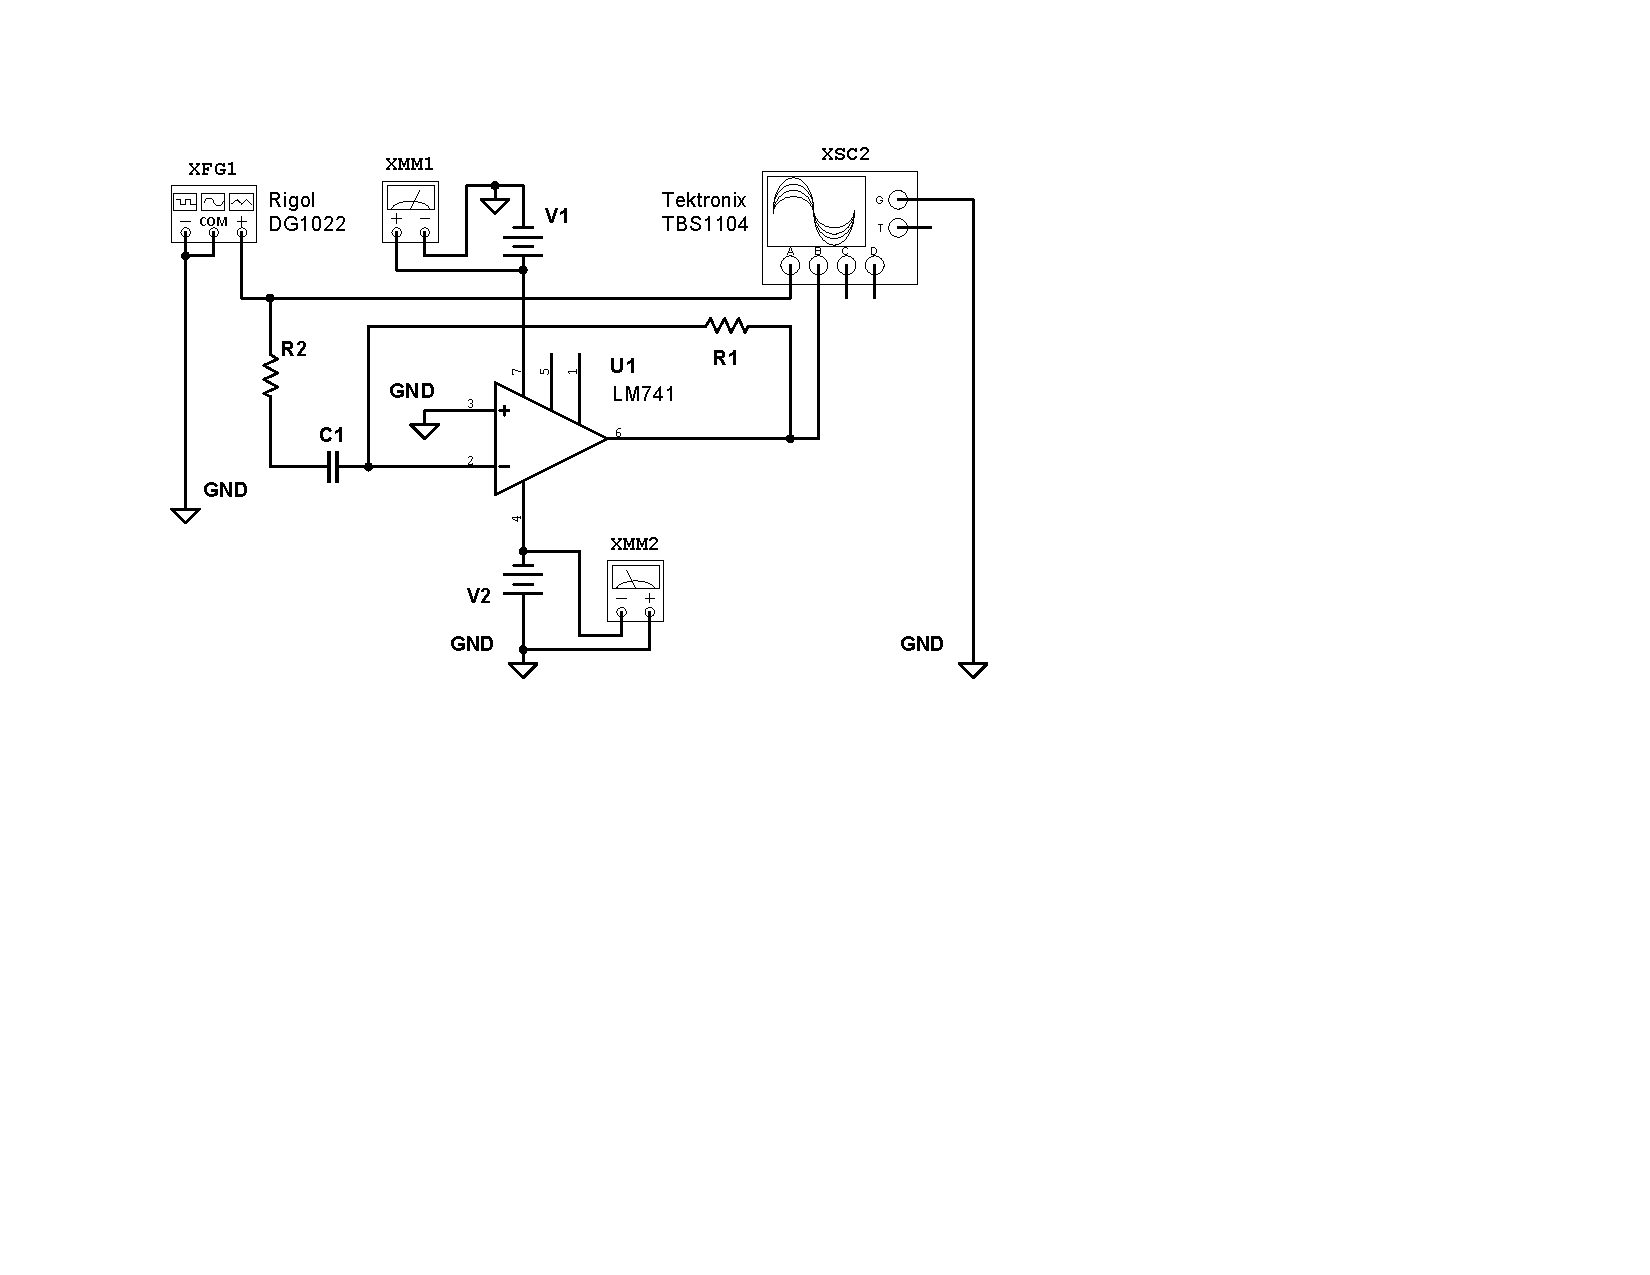
\includegraphics[width=0.38\textwidth]{sch-simulations/output/OPA-deriv.pdf}
\caption{Didascalia}
\label{fig:oscilloscope}
\end {center}
\end{figure}

%%%%%%%%%%FINE SECONDO GIORNO%%%%%%%%%%%%%%%
%%%%%%%%%%INIZIO TERZO GIORNO%%%%%%%%%%%%%%%

%%%%%%%%%%%%%%%%%%%%%%%%%%%%%%%%%%%%%%%%%%
\section{Mixer} %Federico
Sulla \textit{breadboard} è stato implementato il circuito in \textit{fig. 10}. In questa configurazione, l'amplificatore si comporta come circuito sommatore ed il segnale in uscita sarà proporzionale alla somma dei segnali in ingresso. L'OPA è collegato in configurazione invertente, dunque in uscita si otterrà la somma dei segnali cambiata di segno. Nello specifico: 
\[V_{out} = - R  \sum_{n} \frac{V_n}{R_n} = - \sum_{n} V_n\] L'ultimo passaggio è possibile scegliendo tutti i valori delle resistenze uguali ($R = R_1 = R_2$)  

I primi due canali dell'oscilloscopio sono collegati ai segnali $V_1$ e $V_2$ prodotti dal generatore di funzioni, mentre il terzo canale misura la tensione in uscita $V_{out}$.

\begin{figure}[H]%[!ht]
\begin {center}
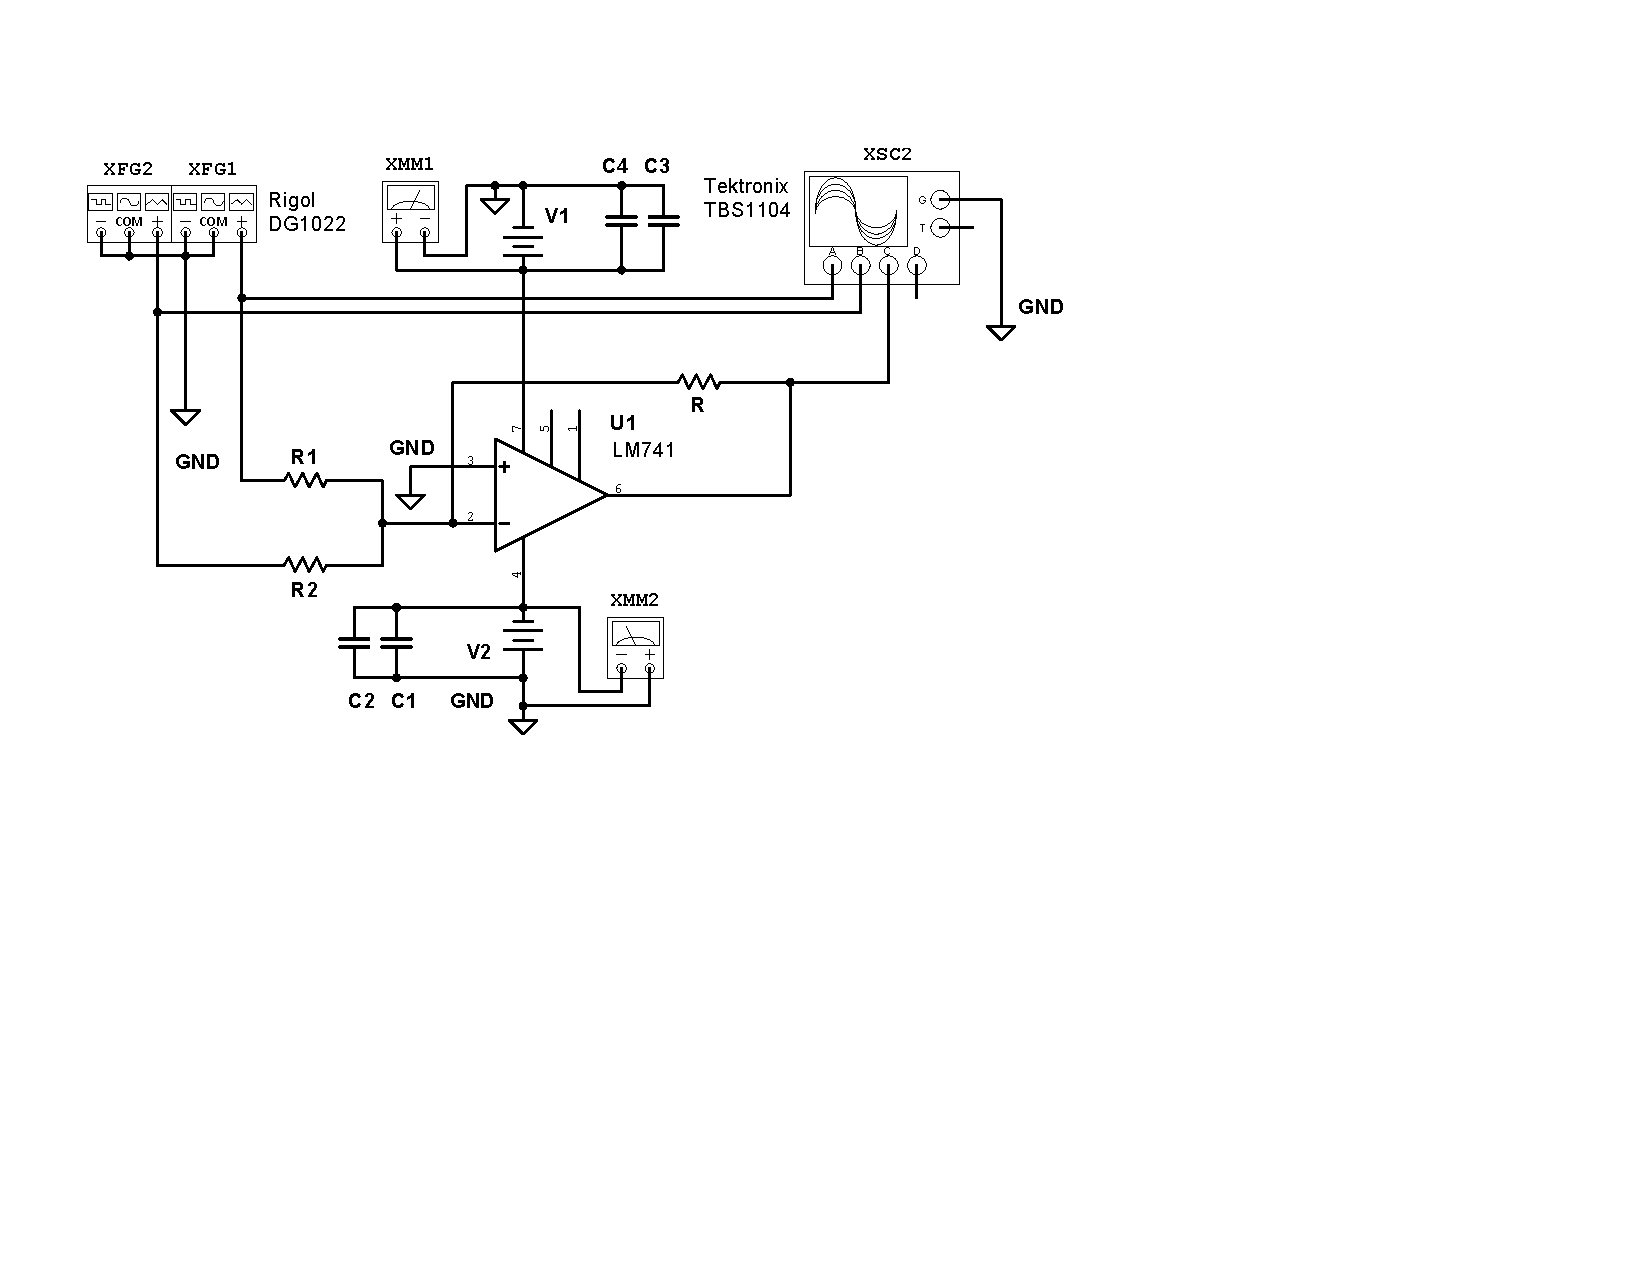
\includegraphics[width=0.38\textwidth]{sch-simulations/output/OPA-mixer.pdf}
\caption{Configurazione invertente del circuito sommatore}
\label{fig:oscilloscope}
\end {center}
\end{figure}

\subsection{Modulazione e battimenti con ingressi sinusoidali}



%%%%%%%%%%%%%%%%%%%%%%%%%%%%%%%%%%%%%%%%%%
\section{Amplificatore di differenze} %Federico
\begin{figure}[H]%[!ht]
\begin {center}
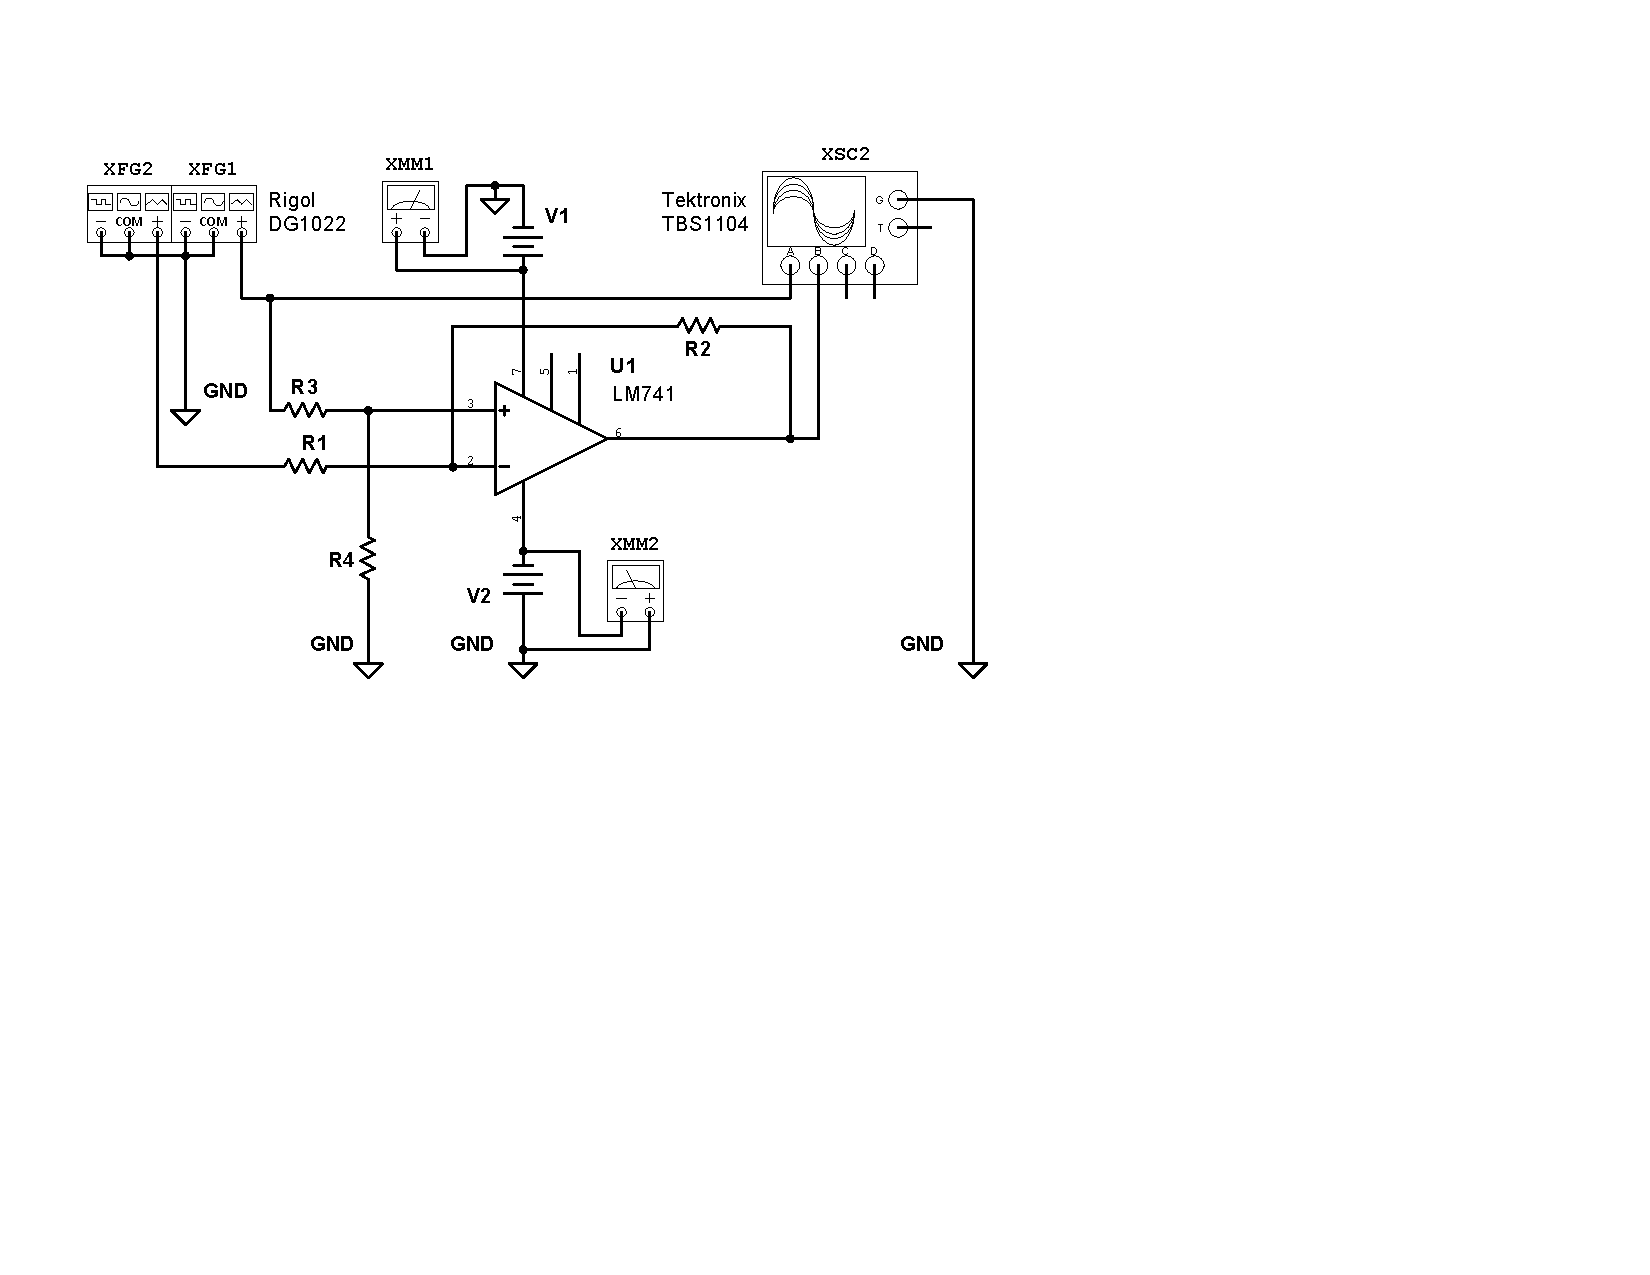
\includegraphics[width=0.38\textwidth]{sch-simulations/output/OPA-difference-amp.pdf}
\caption{Didascalia}
\label{fig:oscilloscope}
\end {center}
\end{figure}

%%%%%%%%%%%%%%%%%%%%%%%%%%%%%%%%%%%%%%%%%%
\section{Trigger di Schmitt} %Federico

\begin{figure}[H]%[!ht]
\begin {center}
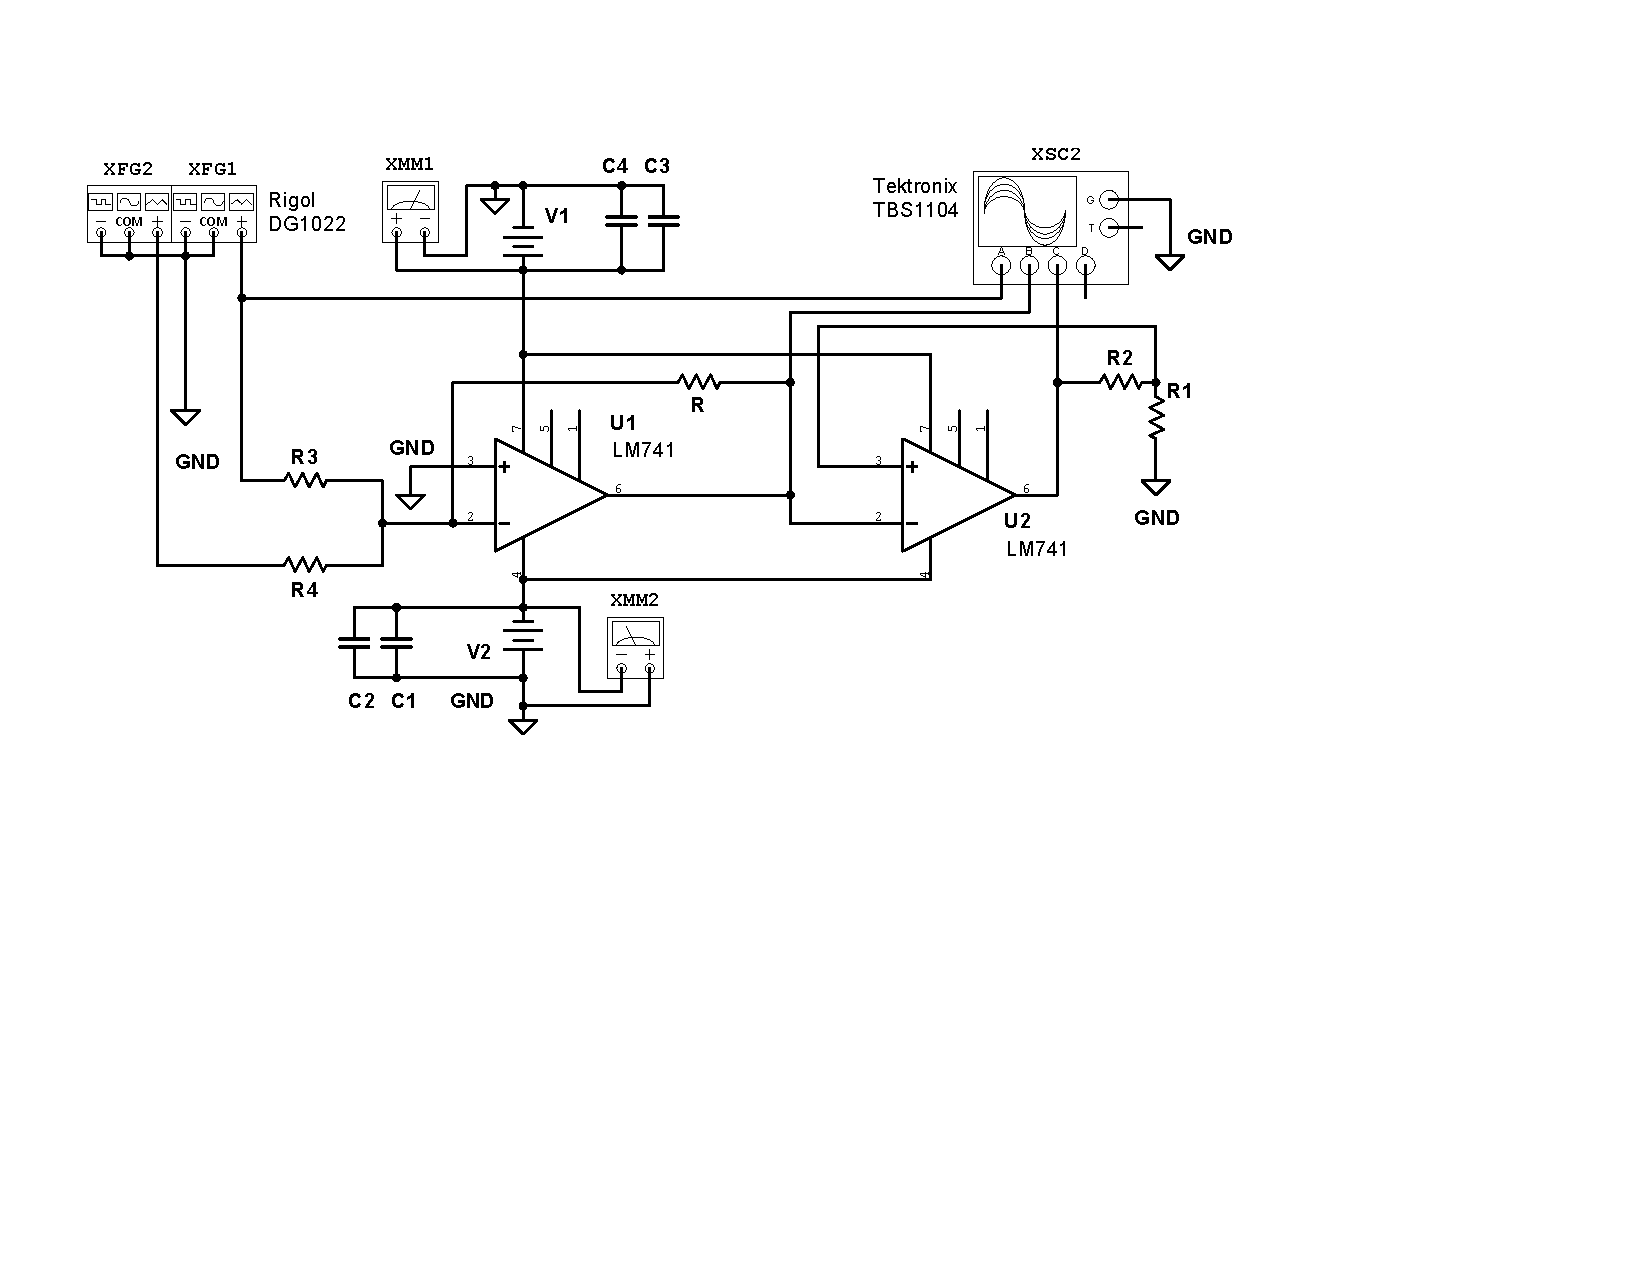
\includegraphics[width=0.48\textwidth]{sch-simulations/output/OPA-mixer-trigger.pdf}
\caption{Didascalia}
\label{fig:oscilloscope}
\end {center}
\end{figure}

\subsection{Ciclo di isteresi al variare della frequenza} %Matteo

%%%%%%%%%%FINE TERZO GIORNO%%%%%%%%%%%%%%%%%%
%%%%%%%%%%INIZIO QUARTO GIORNO%%%%%%%%%%%%%%%

%%%%%%%%%%%%%%%%%%%%%%%%%%%%%%%%%%%%%%%%%%
\section{Silicon photomultiplier} %Valerio
In questa esperienza di laboratorio studieremo qualitativamente il segnale prodotto da un fotomoltiplicatore al silicio illuminato da una sorgente LED. I fotomoltiplicatori al silicio sono fotorivelatori composti da una matrice di SPAD (Single Photon Avalanche Diode) connessi in serie a una resistenza di \textit{quenching} (spegnimento) e collegati in parallelo tra loro. Quando un singolo fotone colpisce il SiPM con una probabilità pari all'efficienza quantica si genera una valanga nello SPAD colpito che provoca un passaggio di corrente dovuto allo scaricamento della capacità di giunzione della cella che provoca una caduta di tensione al catodo (fronte di salita veloce del segnale), al termine della valanga la capacità torna a caricarsi dando origine ad un fronte di discesa più lento. I SiPM sono ampiamente utilizzati per osservare sorgenti di radiazione estremamente deboli o impulsive (anche a livello di singoli fotoni), per esempio nella lettura di rivelatori a scintillazione.

\subsection{Circuito per la caratterizzazione del SiPM}
In laboratorio è stata effettuata una semplice caratterizzazione di due SiPM AdvanSiD NUV: ASD-NUV1S-P e ASD-NUV3S-P caratterizzati da un'efficienza di rilevazione del 43 \%, celle SPAD di dimensione 40x40 $\mu$m, costante di tempo di 70 ns, risposta spettrale tra 350 a 900 nm e guadagno atteso da datasheet di 3.6 $\cdot 10^6$. I due modelli si distinguono per la diversa dimensione della matrice: per il primo 1x1 $mm^2$ (625 celle), mentre per il secondo 3x3 $mm^2$ (5520 celle). Solitamente questi fotorivelatori sono letti in corrente utilizzando un amplificatore transimpedenza, nel nostro caso però si è scelto di impiegare un circuito più semplice, reso possibile dall'elevata sensibilità dell'oscilloscopio Rhode & Schwarz impiegato (fino a 1 mV/div). Il SiPM è stato alimentato con una tensione di polarizzazione di (00.00 $\pm$ 0.0) V (tensione di breakdown $\sim$ 26 V) utilizzando l'alimentatore stabilizzato da laboratorio attraverso tre resistenze di limitazione della corrente come illustrato nello schema seguente, con l'aggiunta di un condensatore di livellamento C1 per ridurre l'eventuale \textit{ripple} dell'alimentazione. Per minimizzare i disturbi esterni la tensione è stata portata dall'alimentatore al circuito mediante un cavo coassiale anziché due cavi di potenza con connettori "a banana". I segnali sono stati portati all'oscilloscopio mediante due condensatori di disaccoppiamento per isolare dalla tensione di \textit{biasing} e i canali sono stati sottratti (essendo tra di loro speculari); questo ha permesso di cancellare parzialmente il rumore dell'alimentazione e di aumentare il \textit{SNR}. Il SiPM è stato illuminato con un led rosso pilotato dal generatore \textit{Siglent SDG1010}.

\begin{figure}[H]%[!ht]
\begin{center}
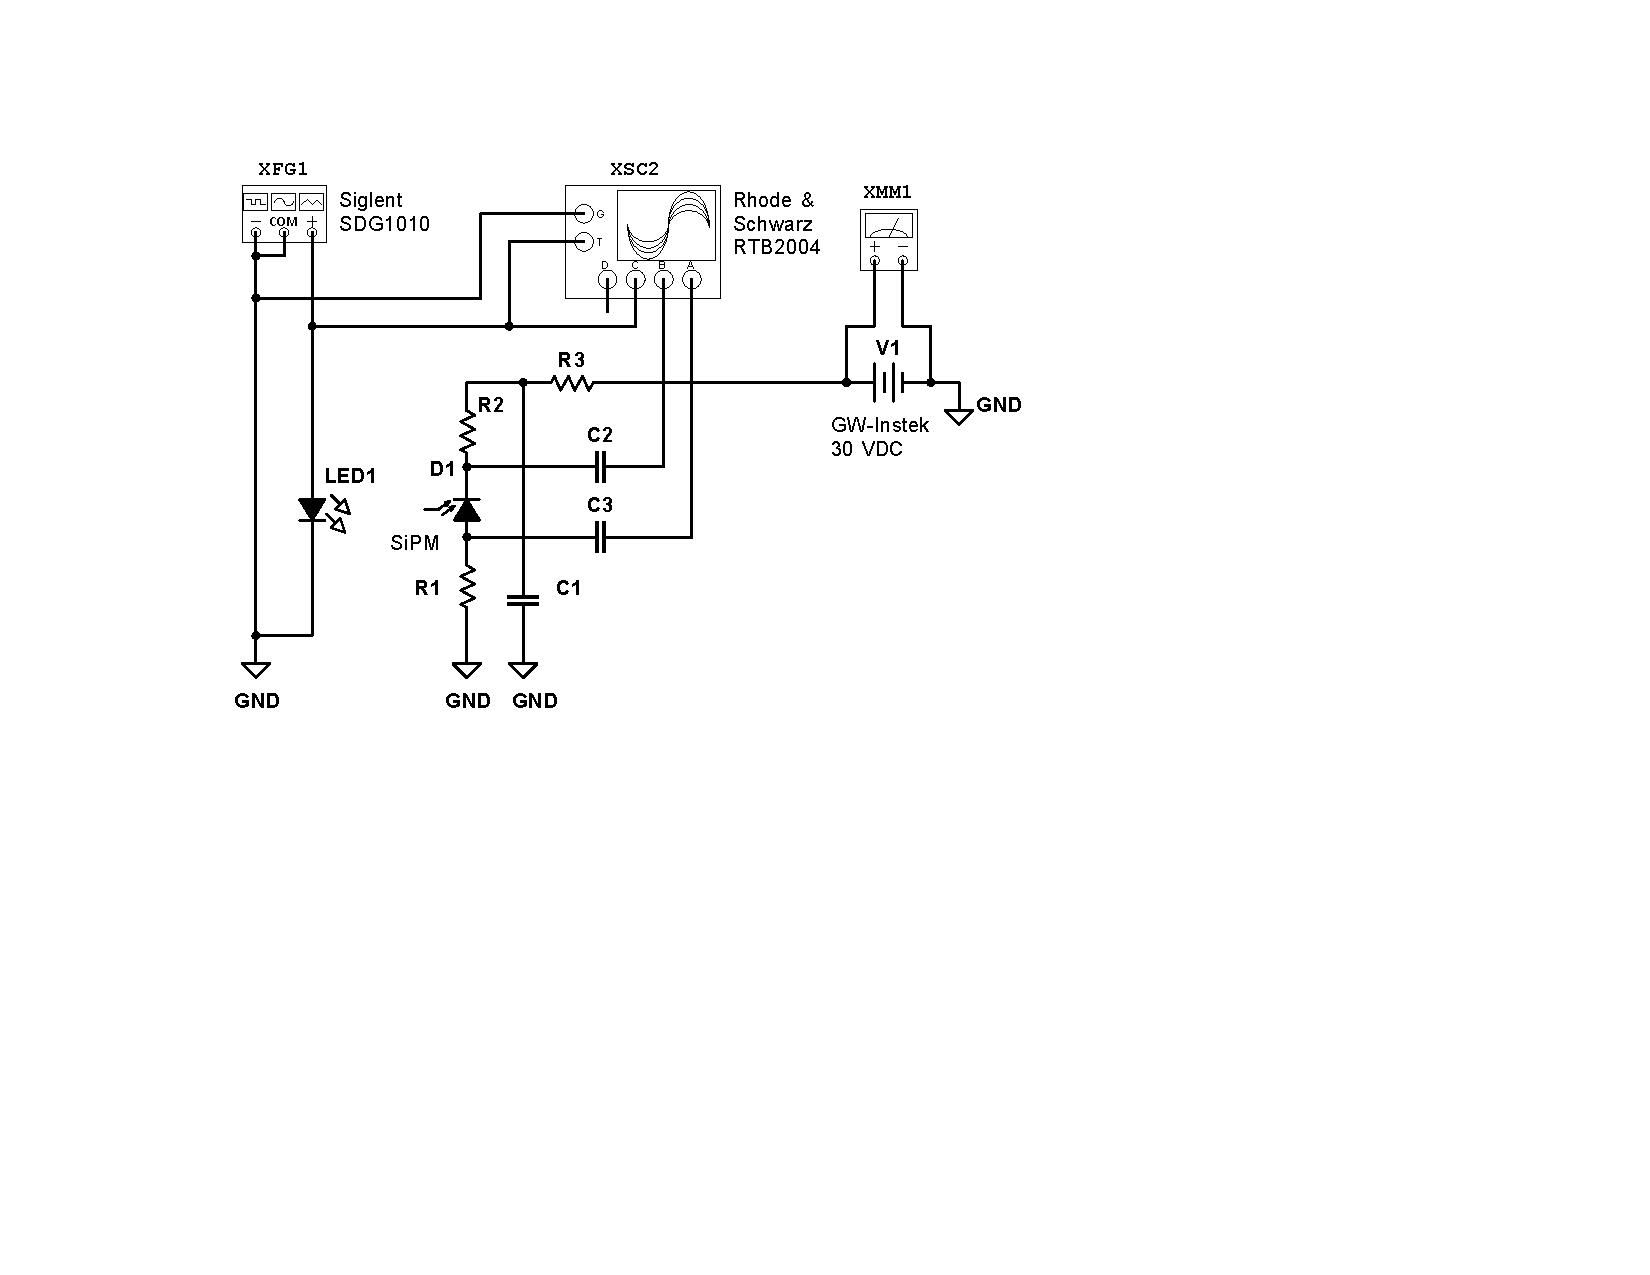
\includegraphics[width=0.46\textwidth]{sch-simulations/output/SiPM.pdf}
\caption{Schema del circuito elettrico per la caratterizzazione del SiPM. Valori per i componenti utilizzati misurati con il multimetro: R1 = (0.00 $\pm$ 0.00) $\Omega$), R2 = (0.00 $\pm$ 0.00) $\Omega$), R3 = (0.00 $\pm$ 0.00) $\Omega$), C1 = (0.00 $\pm$ 0.00) $nF$, C2 = (0.00 $\pm$ 0.00) $nF$, C3 = (0.00 $\pm$ 0.00) $nF$}
\label{fig:oscilloscope}
\end{center}
\end{figure}

\subsection{Funzionamento in saturazione}
Per prima cosa si è proceduto a registrare l'impulso il condizione di saturazione per entrambi i SiPM, cioè l'impulso in uscita prodotto quando tutte le celle vengono eccitate, (dove il numero di celle eccitate è proporzionale al numero di fotoni rivelati). Per studiare questo aspetto è stata aumentata l'ampiezza dell'impulso di pilotaggio del LED fino a 0.000 V (durata $\Delta$t = 16 ns, frequenza di ripetizione $f$ = 0.00 KHz) per il sensore 1x1 $mm^2$ e 0.000 V per il sensore 3x3 $mm^2$. I risultati sono presentati nei grafici in figura \ref{fig:SiPM_sat_1mm} e \ref{fig:SiPM_sat_3mm} rispettivamente. Notiamo come l'impulso del SiPM di dimensioni maggiori sia più prolungato, di ampiezza maggiore e più rumoroso, questi effetti sono conseguenza naturale di un numero maggiore di celle SPAD, in particolare la maggiore durata è dovuta ad una più elevata capacità parassita dovuta alla presenza di molte più celle in parallelo.


\begin{figure}[H]%[!ht]
\begin{center}
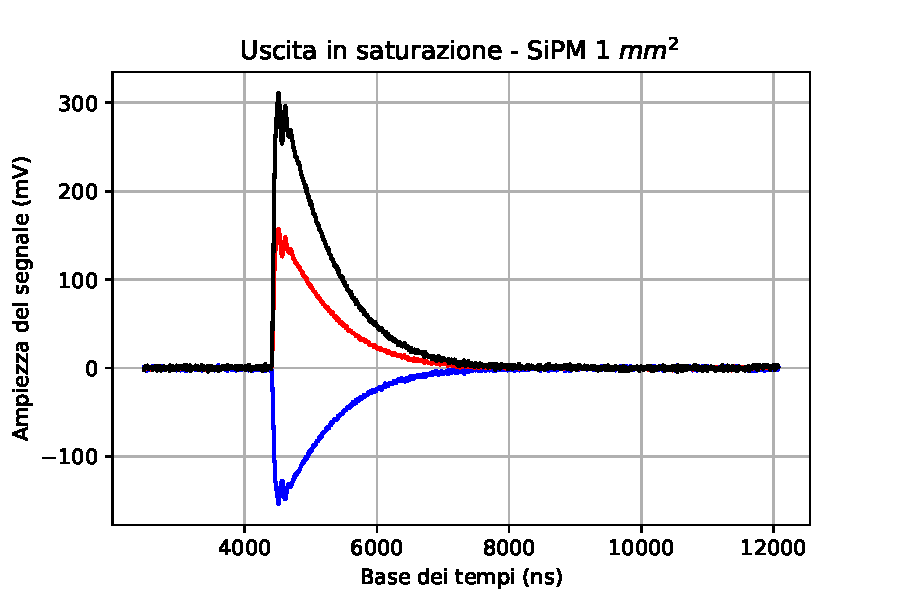
\includegraphics[width=0.40\textwidth]{analysis/output/SiPM_sat_1mm.pdf}
\caption{Segnale prodotto dal SiPM 1x1 $mm^2$ in saturazione: in rosso la tensione all'anodo, il blu la tensione al catodo, il nero la differenza calcolata dall'oscilloscopio.}
\label{fig:SiPM_sat_1mm}
\end{center}
\end{figure}

\begin{figure}[H]%[!ht]
\begin{center}
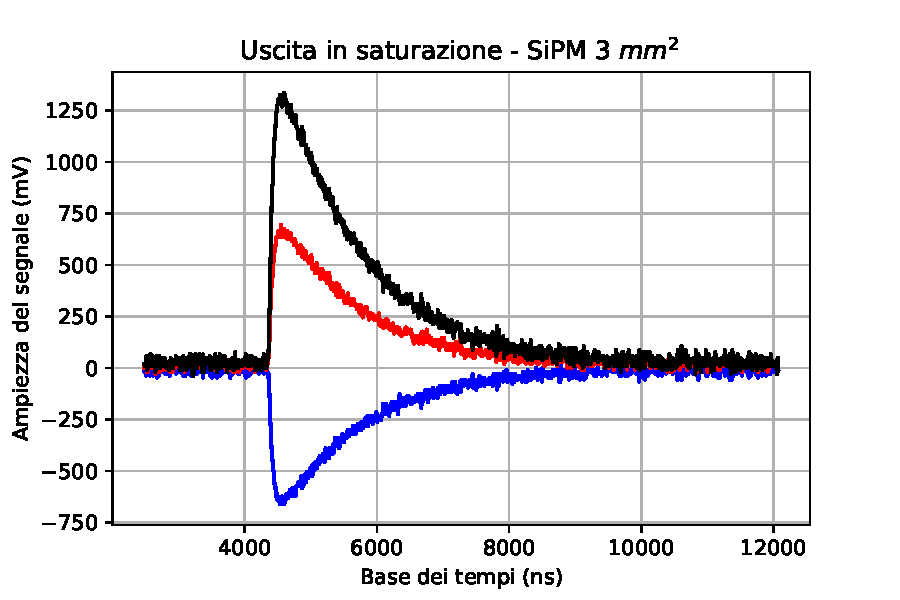
\includegraphics[width=0.40\textwidth]{analysis/output/SiPM_sat_3mm.pdf}
\caption{Segnale prodotto dal SiPM 3x3 $mm^2$ in saturazione: in rosso la tensione all'anodo, il blu la tensione al catodo, il nero la differenza calcolata dall'oscilloscopio.}
\label{fig:SiPM_sat_3mm}
\end{center}
\end{figure}

\subsection{Valutazione del guadagno e del tempo di carica caratteristico}
In questa fase, più delicata, si vuole invece valutare il guadagno di ciascuna cella e calcolare il tempo caratteristico di carica, dipendente dalla resistenza totale della cella e dalla capacità parassita, che compongono una rete RC. Per raggiungere questo obiettivo si vuole visualizzare una sovrapposizione di impulsi dovuti dall'attivazione di esattamente 1, 2, 3, ... N celle e poter calcolare la differenza in tensione tra i picchi di questi impulsi. Configuriamo allora il generatore il modo da produrre impulsi di bassissima intensità (stesse impostazioni di prima, ma V = 0.000 mV) in modo che ciascun impulso produca un numero esiguo di fotoni che provocherà l'accensione di poche celle, secondo un modello poissoniano e impostiamo correttamente la persistenza delle tracce sull'oscilloscopio. Si ottengono così i grafici nelle figure \ref{fig:staircase_1mm} e \ref{fig:staircase_3mm} per i due SiPM. A partire da tali tracce sono stati ricavati i valori di tensione di picco per ciascun impulso corrispondente ad un determinato numero di celle con metodi numerici.

\begin{figure*}[t]%[t]
\centering
\begin{center}
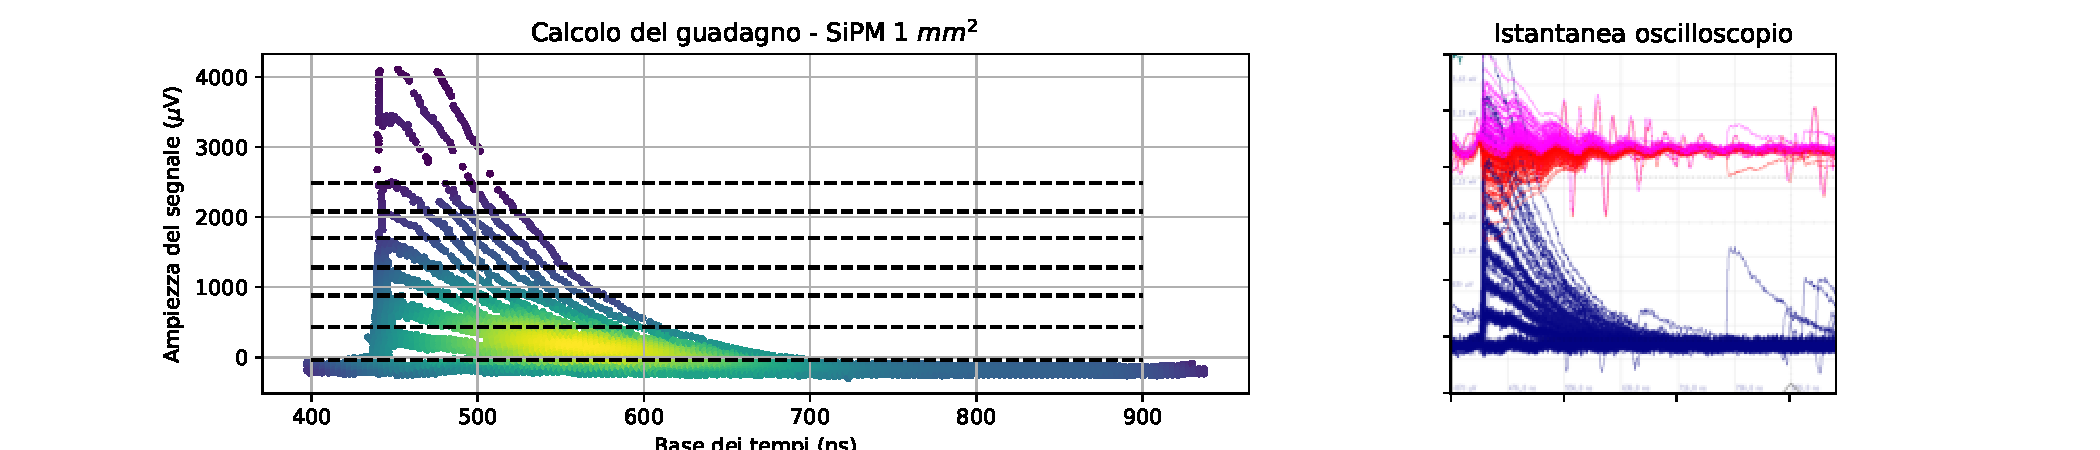
\includegraphics[width=1.05\textwidth]{analysis/output/SiPM_1mm_gain_staircase.pdf}
\end{center}
\caption{A destra l'istantanea catturata dallo schermo dell'oscilloscopio, a sinistra le tracce estratte numericamente sovrapposte con i cursori orizzontali corrispondenti alle tensioni di picco per l'attivazione di N celle. Il gradiente di colore rappresenta invece la densità di tracce. SiPM 1x1 $mm^2$}
\label{fig:staircase_1mm}
\end{figure*}

\begin{figure*}[t]%[t]
\centering
\begin{center}
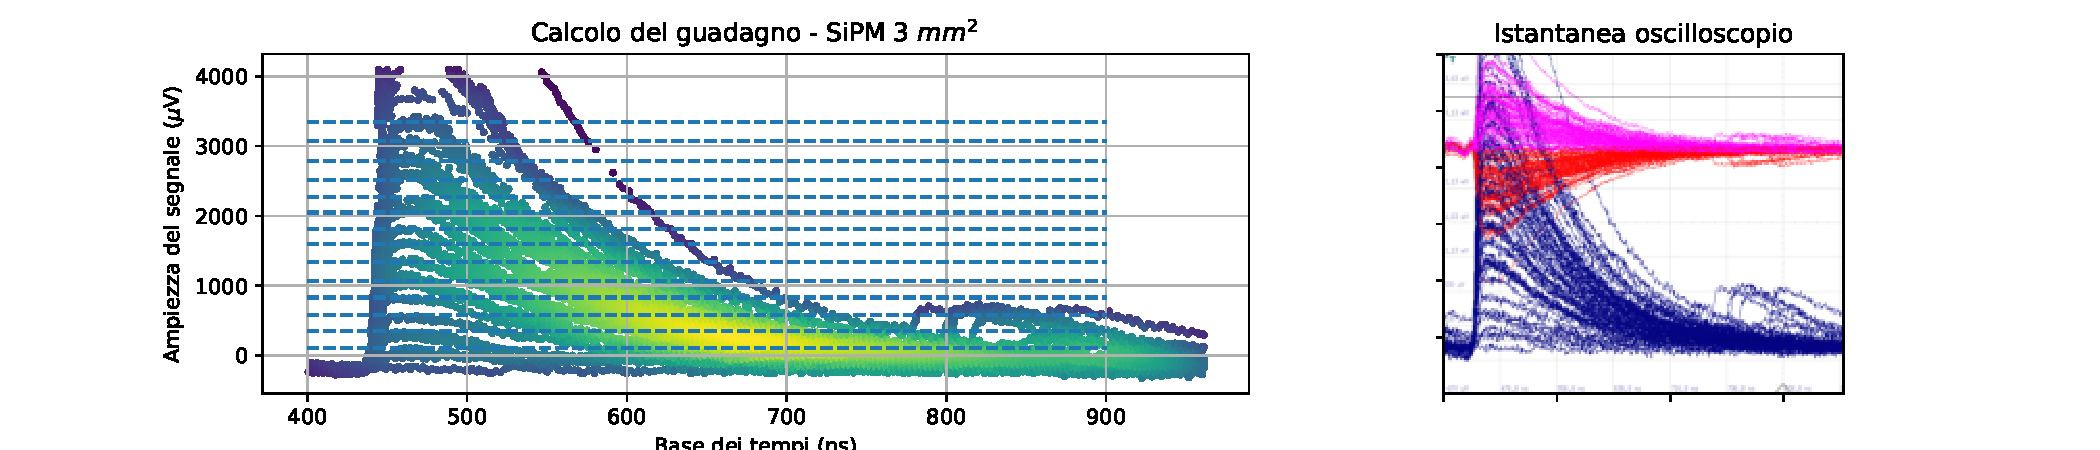
\includegraphics[width=1.05\textwidth]{analysis/output/SiPM_3mm_gain_staircase.pdf}
\end{center}
\caption{Come nella figura precedente, ma questa volta per il SiPM di dimensioni 3x3 $mm^2$}
\label{fig:staircase_3mm}
\end{figure*}

\subsection{Discussione e considerazioni conclusive}
Testo

%%%%%%%%%%%%%%%%%%%%%%%%%%%%%%%%%%%%%%%%%%
\section{Linea di ritardo} %Federico

\section{Silicon photomultiplier} %Valerio

\begin{figure}[H]%[!ht]
\begin {center}
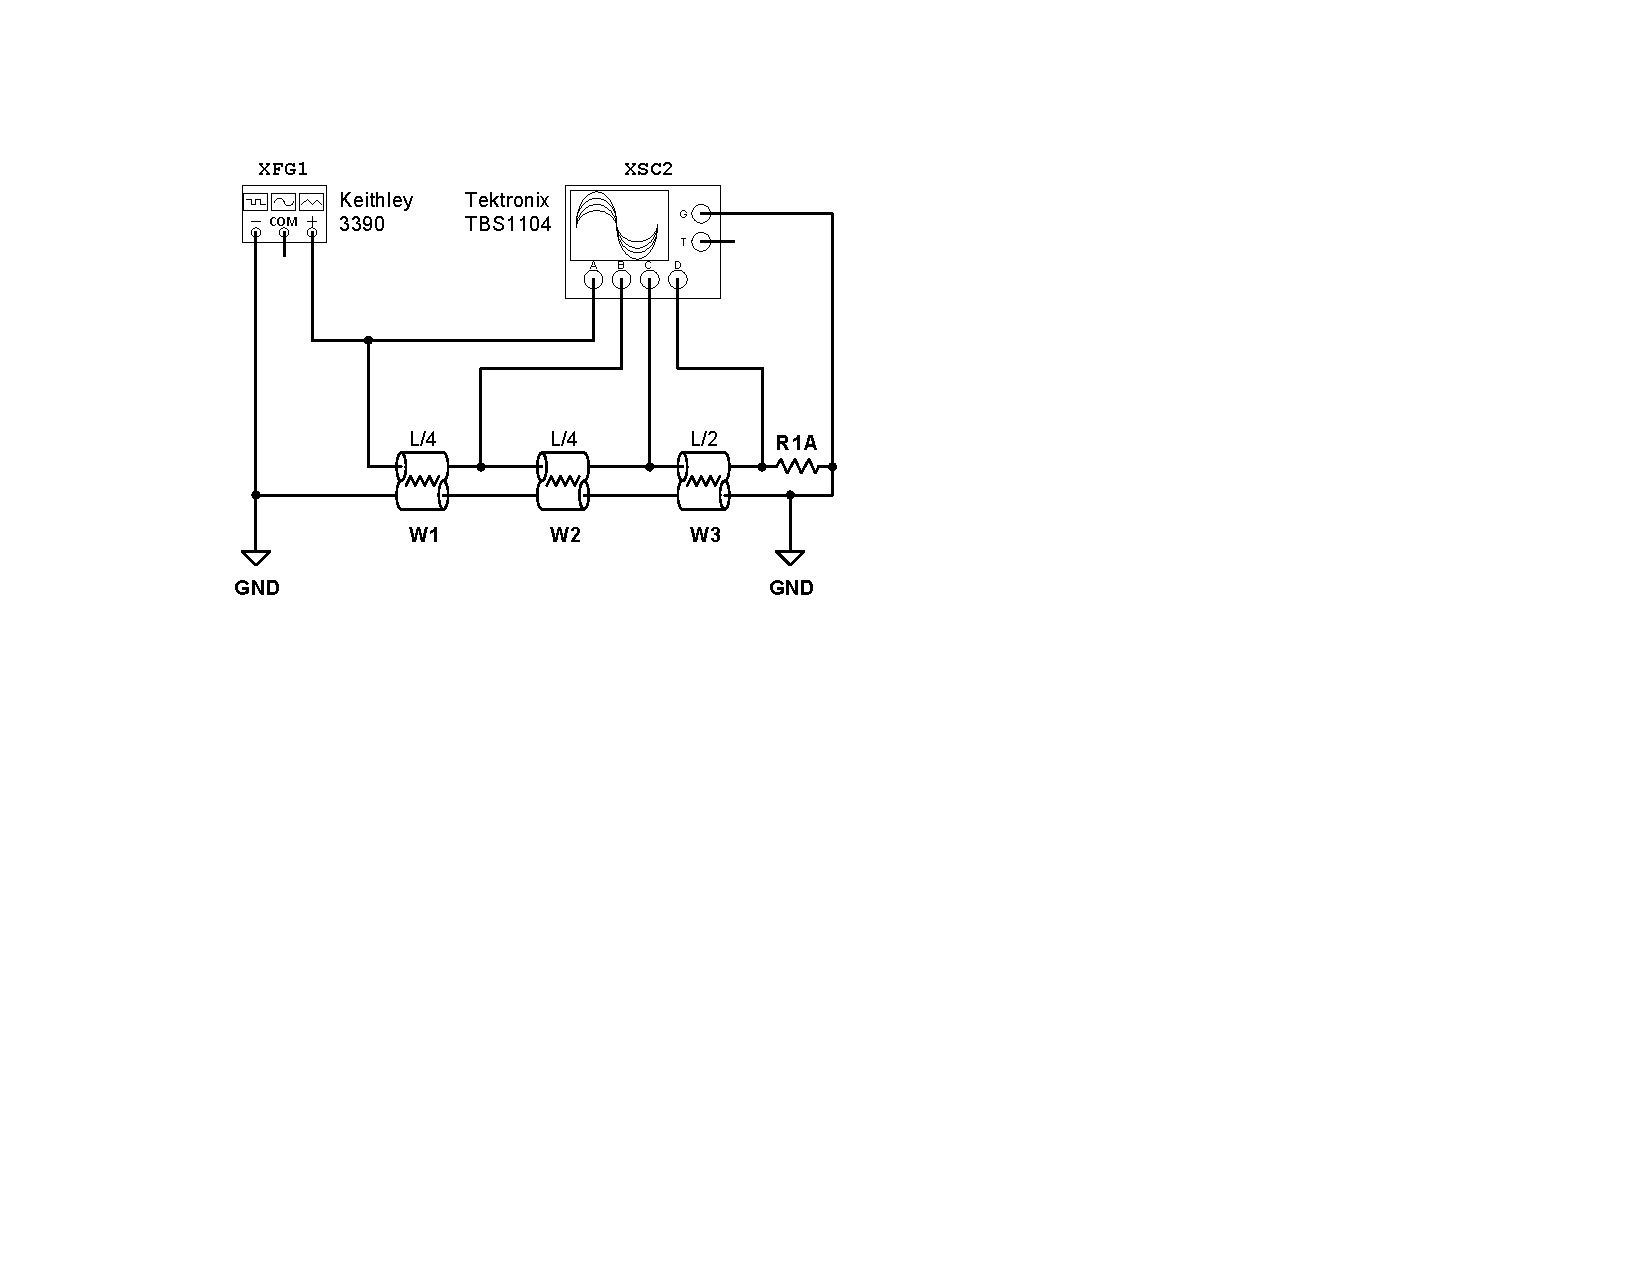
\includegraphics[width=0.38\textwidth]{sch-simulations/output/Transmission line.pdf}
\caption{Didascalia}
\label{fig:oscilloscope}
\end {center}
\end{figure}

\subsection{Tempo di volo impulso singolo}

\subsection{Repetition rate e frequenza di accordatura}

\subsection{Formazione di onde stazionarie}

\subsection{Armoniche 2L}

\subsection{Armoniche L}

%%%%%%%%%%%%%%%%%%%%%%%%%%%%%%%%%%%%%%%%%%
\section{Conclusioni generali} %Tutti quanti


%%%%%%%%%%%%%%%%%%%%%%%%%%%%%%%%%%%%%%%%%%
\section{Appendice}


%%%%%%%%%%%%%%%%%%%%%%%%%%%%%%%%%%%%%%%%%%
\section{Riferimenti}
\printbibliography

%%%%%%%%%%%%%%%%%%%%%%%%%%%%%%%%%%%%%%%%%%
\section{Indice}
\tableofcontents


\end{document}


